\documentclass[10pt]{beamer}
% \usetheme{Boadilla}
  \usetheme{default}


% acronyms for text or math mode
\newcommand {\ccast} {\mbox{\small\textsc{ccast}}}
\newcommand {\kcarta} {\mbox{k\small{CARTA}}}

\newcommand {\cris} {\mbox{\small CrIS}}
\newcommand {\airs} {\mbox{\small AIRS}}
\newcommand {\iasi} {\mbox{\small IASI}}
\newcommand {\idps} {\mbox{\small IDPS}}
\newcommand {\nasa} {\mbox{\small NASA}}
\newcommand {\noaa} {\mbox{\small NOAA}}
\newcommand {\nstar} {\mbox{\small STAR}}
\newcommand {\umbc} {\mbox{\small UMBC}}
\newcommand {\uw}   {\mbox{\small UW}}

\newcommand {\fft}  {\mbox{\small FFT}}
\newcommand {\ifft} {\mbox{\small IFFT}}
\newcommand {\fir}  {\mbox{\small FIR}}
\newcommand {\fov}  {\mbox{\small FOV}}
\newcommand {\for}  {\mbox{\small FOR}}
\newcommand {\ict}  {\mbox{\small ICT}}
\newcommand {\ils}  {\mbox{\small ILS}}
\newcommand {\igm}  {\mbox{\small IGM}}
\newcommand {\opd}  {\mbox{\small OPD}}
\newcommand {\rms}  {\mbox{\small RMS}}
\newcommand {\zpd}  {\mbox{\small ZPD}}
\newcommand {\ppm}  {\mbox{\small PPM}}
\newcommand {\srf}  {\mbox{\small SRF}}
\newcommand {\sdr}  {\mbox{\small SDR}}
\newcommand {\FWHM} {\mbox{\small FWHM}}
\newcommand {\fwhm} {\mbox{\small\textsc{fwhm}}}

\newcommand {\ES} {\mbox{\small ES}}
\newcommand {\SP} {\mbox{\small SP}}
\newcommand {\IT} {\mbox{\small IT}}
\newcommand {\SA} {\mbox{\small SA}}

\newcommand {\ET} {\mbox{\small ET}}
\newcommand {\FT} {\mbox{\small FT}}

\newcommand {\wn} {\mbox{cm$^{-1}$}}
\newcommand {\cm} {\mbox{cm}}

% abbreviations, mainly for math mode
\newcommand {\real} {\mbox{real}}
\newcommand {\imag} {\mbox{imag}}
\newcommand {\atan} {\mbox{atan}}
\newcommand {\obs}  {\mbox{obs}}
\newcommand {\calc} {\mbox{calc}}
\newcommand {\sinc} {\mbox{sinc}}
\newcommand {\psinc} {\mbox{psinc}}
\newcommand {\std} {\mbox{std}}

% symbols, for math mode only
\newcommand {\lmax} {L_{\mbox{\tiny max}}}
\newcommand {\vmax} {V_{\mbox{\tiny max}}}

\newcommand {\tauobs} {\tau_{\mbox{\tiny obs}}}
\newcommand {\taucal} {\tau_{\mbox{\tiny calc}}}
\newcommand {\Vdc}  {V_{\mbox{\tiny DC}}}

\newcommand {\rIT} {r_{\mbox{\tiny\textsc{ict}}}}
\newcommand {\rES} {r_{\mbox{\tiny\textsc{es}}}}
\newcommand {\robs} {r_{\mbox{\tiny obs}}}

\newcommand {\rITobs} {r_{\mbox{\tiny\textsc{ict}}}^{\mbox{\tiny obs}}}
\newcommand {\rITcal} {r_{\mbox{\tiny\textsc{ict}}}^{\mbox{\tiny cal}}}

\newcommand {\rESuser} {r_{\mbox{\tiny\textsc{es}}}^{\mbox{\tiny user}}}
\newcommand {\rITuser} {r_{\mbox{\tiny\textsc{ict}}}^{\mbox{\tiny user}}}
\newcommand {\rITsensor} {r_{\mbox{\tiny\textsc{ict}}}^{\mbox{\tiny sensor}}}
\newcommand {\rITfov} {r_{\mbox{\tiny\textsc{ict}}}^{\mbox{\tiny fov}}}

\newcommand {\fcos} {f_{\mbox{\tiny cos}}}
\newcommand {\fatbd} {f_{\mbox{\tiny\textsc{atbd}}}}

\newcommand {\ITmean} {\langle\mbox{\small IT}\rangle}
\newcommand {\SPmean} {\langle\mbox{\small SP}\rangle}

\newcommand {\Ttc} {t^{\mbox{\tiny\textsc{tc}}}}
\newcommand {\Tac} {t^{\mbox{\tiny\textsc{ac}}}}
\newcommand {\rtc} {r_{\mbox{\tiny\textsc{tc}}}}
\newcommand {\rta} {r_{\mbox{\tiny\textsc{ta}}}}



\title{A first look at the Jan 2020\\
  CrIS TVAC PFH gas cell tests}
\author{H.~E.~Motteler, L.~L.~Strow, \\
  S.~DeSouza-Machado, \\
  S.~Buczkowski
}
\institute{
  UMBC Atmospheric Spectroscopy Lab \\
  Joint Center for Earth Systems Technology \\
}
\date{\today}
\begin{document}

%----------- slide --------------------------------------------------%
\begin{frame}[plain]
\titlepage
\end{frame}
%----------- slide --------------------------------------------------%
\begin{frame}
\frametitle{Introduction}
\begin{itemize}

  \item We present a preliminary analysis of the PFH Plateau 21
    CH$_4$, CO$_2$, and CO gas cell tests, and compare these with
    calculated reference truth from LBLRTM and UMBC-LBL.

  \item We have also done a reanalysis of the PFL Plateau 20 test
    with more careful harvesting of the individual test legs and
    more accurate calculated transmittances.  The resulting changes
    to the metrology laser relative residuals were less than 1 ppm.
 
   \item Examples of monitoring test logs (the CSS, CMD, and TCR
     files) are given in the form of plots of HTBB temperature, gas
     cell temperature, and gas cell pressure over time.

  \item The J2 tests continue to be done at the older 866/1052/799
    point resolutions.
    
\end{itemize}
\end{frame}
%----------- slide --------------------------------------------------%
\begin{frame}
\frametitle{Methods}
\begin{itemize}

  \item For each gas we partition the data stream into four test
    legs, \\ FT1, FT2, ET1, and ET2 (cell full, HTBB temperature T1,
    etc.)

  \item For test each leg, we take the mean of the associated count
    spectra, calculate the transmittance as $(FT2 - FT1) / (ET2 -
    ET1)$, apply our standard processing filters, and do the SA
    correction, all at the sensor grid.  Expected transmittance
    values are also calculated at the sensor grid.

  \item This is similar in some ways to the ``ratio first''
    calibration algorithm used as an option in UMBC CCAST
    processing, but note that we do not do a full radiance
    calibration, or any nonlinearity correction, for the analysis
    here.

  \item Measured and calculated transmittances are compared first as
    is, and then by fitting obs to calcs and examining fitting
    weights and residuals.

  \item This approach, with fitting adjustments, is acceptable for
    our application because our main task is spectral calibration
    and our fitting methods are robust in the face of radiometric
    uncertainty.

\end{itemize}
\end{frame}
%----------- slide --------------------------------------------------%
\begin{frame}
\frametitle{12-13 Jan 2020 TVAC PFH Plateau 21}
\begin{columns}[t]
\begin{column}{0.5\textwidth}
  \begin{centering}
  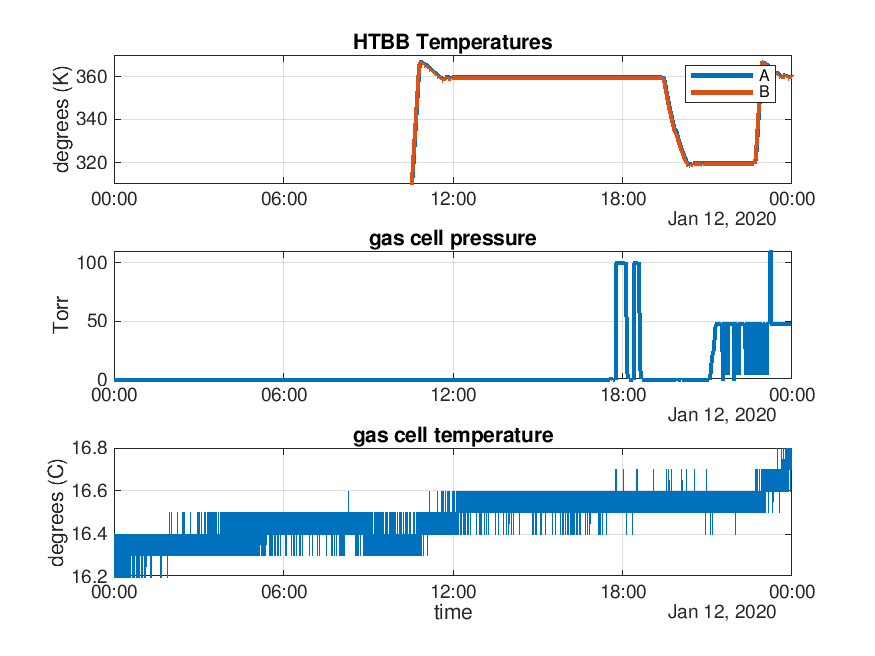
\includegraphics[width=\textwidth]{harvest_01-12/css_summary_12_jan.png}
  \end{centering}\vspace{3mm}

\end{column}
\begin{column}{0.5\textwidth}  
  \begin{centering}
  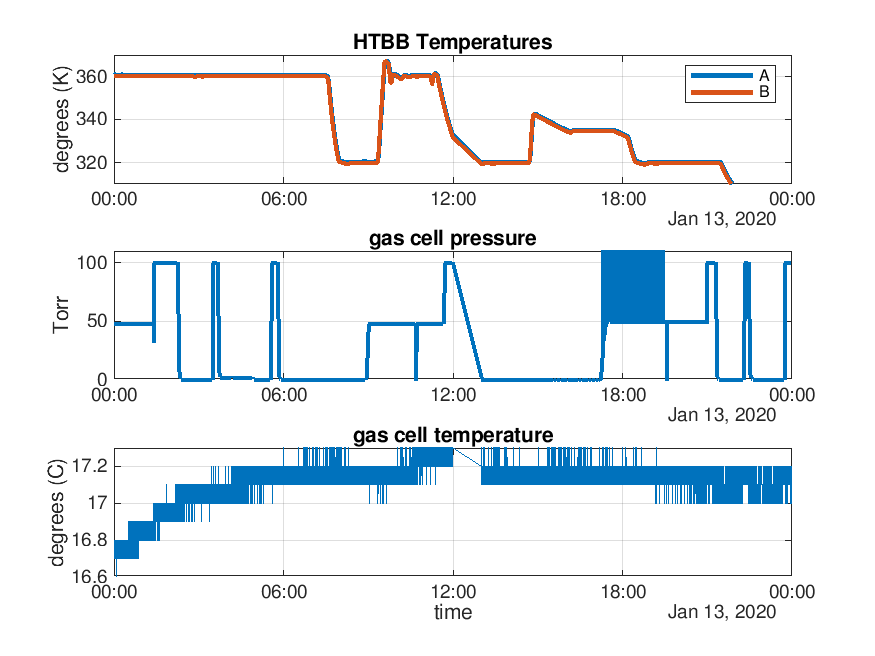
\includegraphics[width=\textwidth]{harvest_01-12/css_summary_13_jan.png}
  \end{centering}\vspace{3mm}

\end{column}
\end{columns}

HTBB temperatures, gas cell pressure and gas cell temperature from
the CCS files, for 12-13 Jan 2020.  This data is used along with a
scan of the CMD and SQL files for an overview and to find the test
stages. 

\end{frame}
%----------- slide --------------------------------------------------%
\begin{frame}
\frametitle{19 Jan 2020 TVAC PFH Plateau 21}
\begin{columns}[t]
\begin{column}{0.6\textwidth}
  \begin{centering}
  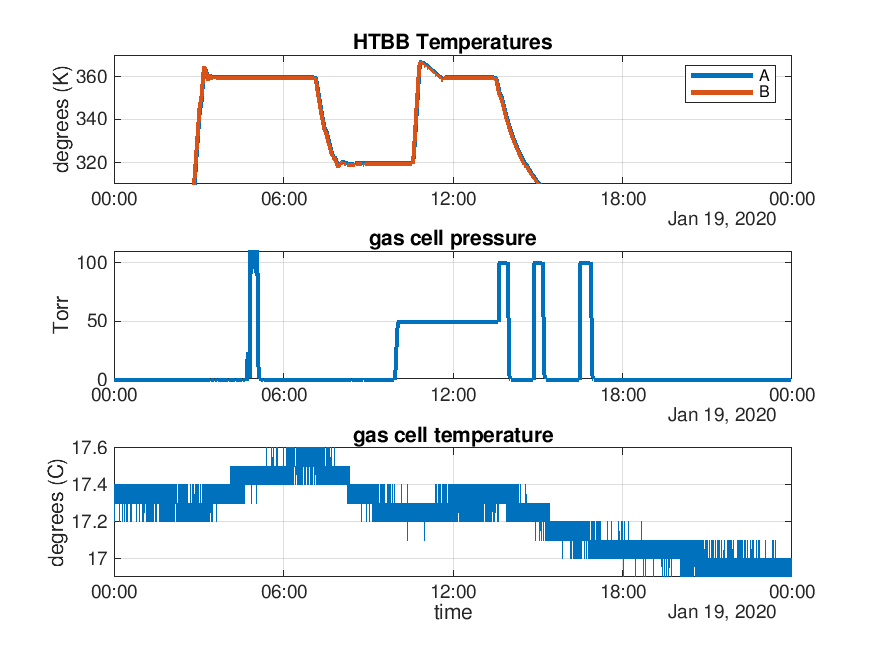
\includegraphics[width=\textwidth]{harvest_01-19/css_summary_19_jan.png}
  \end{centering}\vspace{3mm}

% \end{column}
% \begin{column}{0.5\textwidth}  
%   \begin{centering}
%   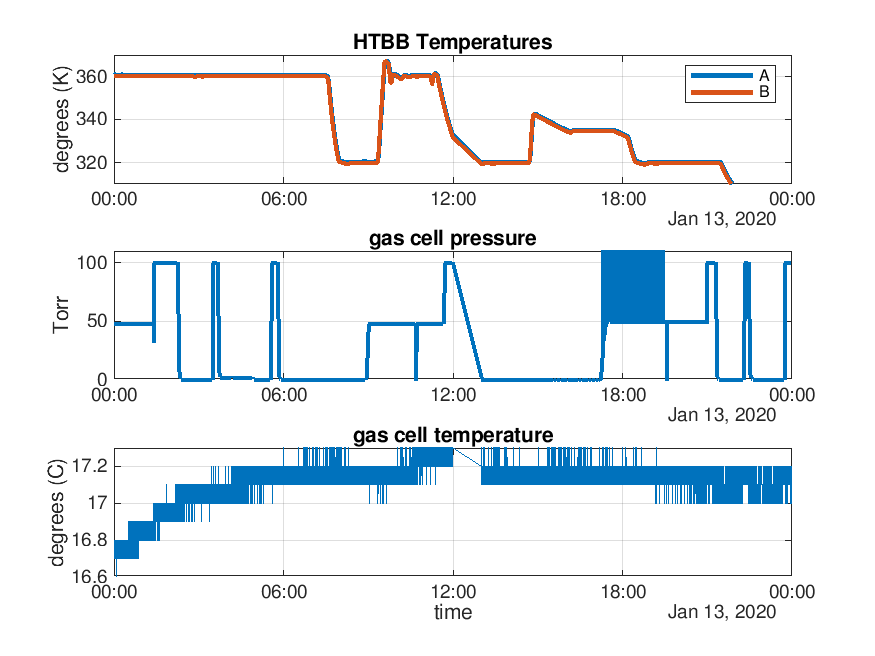
\includegraphics[width=\textwidth]{harvest_01-12/css_summary_13_jan.png}
%   \end{centering}\vspace{3mm}

\end{column}
\end{columns}

HTBB temperatures, gas cell pressure and gas cell temperature from
the CCS files, for 19 Jan 2020.  This data is used along with a scan
of the CMD and SQL files for an overview and to find the test stages.

\end{frame}
%----------- slide --------------------------------------------------%
\begin{frame}
\frametitle{CO$_2$ LW PFH side 1 test parameters}

\begin{itemize}
  \item PFH Plateau 21, 12 Jan 2019
  \item side 1, sweep direction 0
  \item fitting interval 672 to 712 $\wn$
  \item metrology laser 774.22556 nm, from neon 703.44765 nm
  \item ATBD default focal plane
  \item SA correction from ILS with periodic sinc at the sensor grid
  \item HTBB nominal T1 360 K, T2 320 K
  \item gas cell pressure 48.36 Torr
  \item gas cell temperature 16.65 C
  \item gas cell length 12.59 cm
\end{itemize}

\end{frame}
%----------- slide --------------------------------------------------%
\begin{frame}
\frametitle{CO$_2$ PFH side 1 cell empty test legs}
\begin{columns}[t]
\begin{column}{0.5\textwidth}
  \begin{centering}
  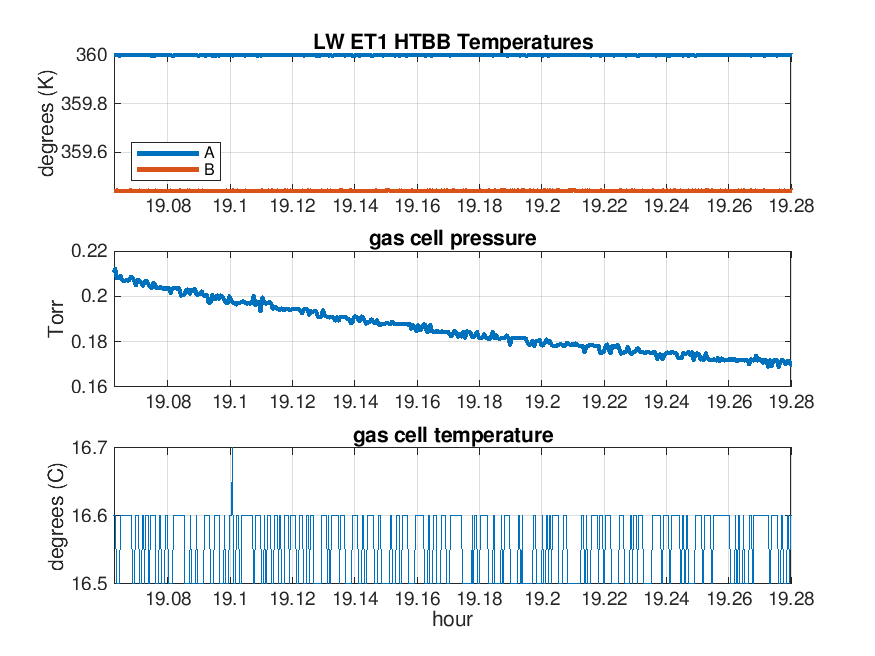
\includegraphics[width=\textwidth]{harvest_01-12/01-12_LW_ET1.png}
  \end{centering}\vspace{3mm}

  ET1 ``empty high'' leg of the the 12 Jan CO$_2$ transmittance test.
  The x-axis here is hour of the day.  The HTBB temps are stable but
  we see a vestigal pressure drift.

\end{column}
\begin{column}{0.5\textwidth}  
  \begin{centering}
  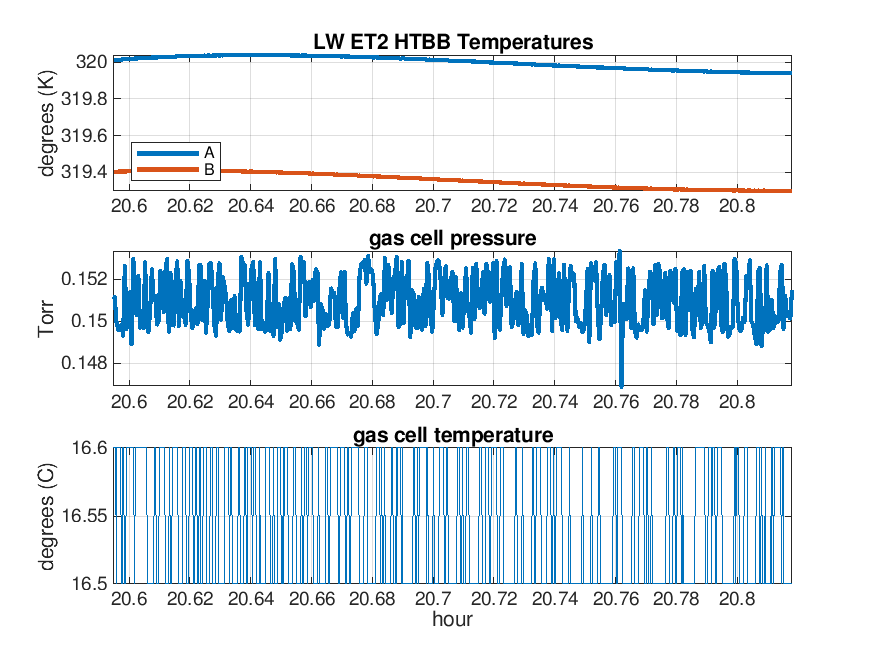
\includegraphics[width=\textwidth]{harvest_01-12/01-12_LW_ET2.png}
  \end{centering}\vspace{3mm}

  ET2 ``empty low'' leg of the the 13 Jan CO$_2$ transmittance test.
  We see some HTBB drift.

\end{column}
\end{columns}
\end{frame}
%----------- slide --------------------------------------------------%
\begin{frame}
\frametitle{CO$_2$ PFH side 1 cell full test legs}
\begin{columns}[t]
\begin{column}{0.5\textwidth}
  \begin{centering}
  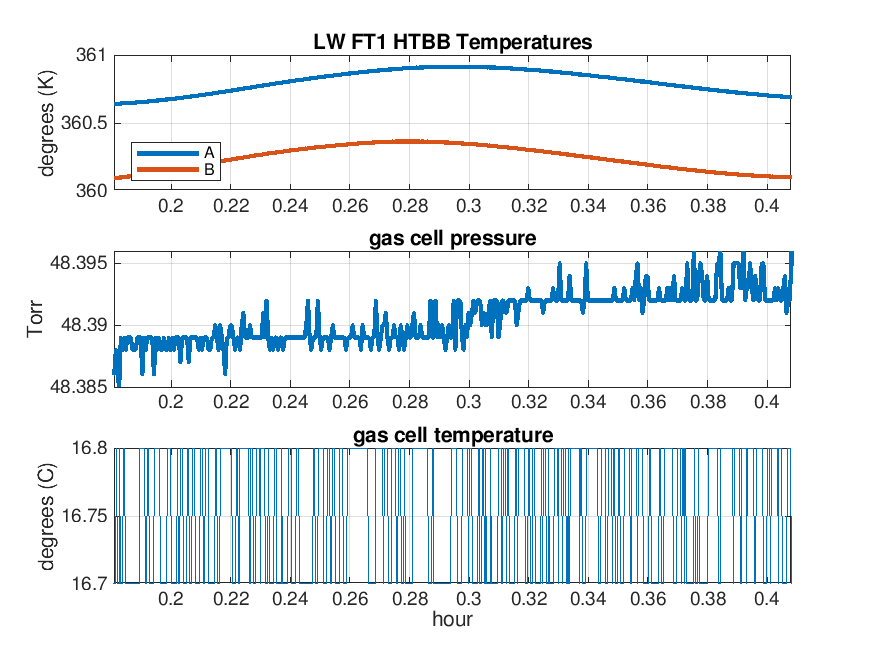
\includegraphics[width=\textwidth]{harvest_01-12/01-12_LW_FT1.png}
  \end{centering}\vspace{3mm}

  FT1 ``full high'' leg of the the 12 Jan CO$_2$ transmittance test.
  The x-axis is hour of the day.  As in the empty low leg we see
  some HTBB drift.

\end{column}
\begin{column}{0.5\textwidth}  
  \begin{centering}
  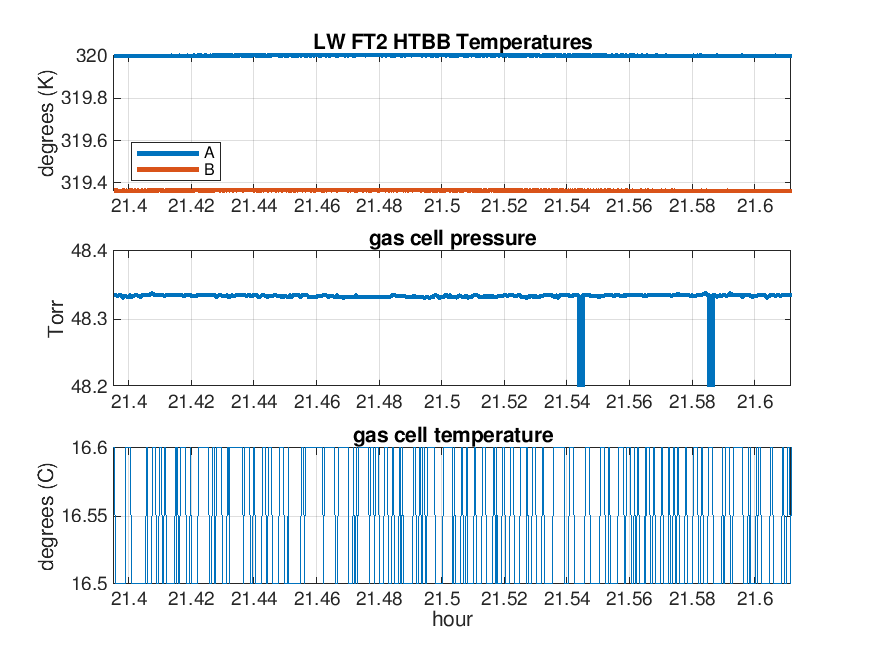
\includegraphics[width=\textwidth]{harvest_01-12/01-12_LW_FT2.png}
  \end{centering}\vspace{3mm}

  FT2 ``full low'' leg of the the 12 Jan CO$_2$ transmittance test.
  This looks good.

\end{column}
\end{columns}
\end{frame}
%----------- slide --------------------------------------------------%
\begin{frame}
\frametitle{CO$_2$ side 1 data before fitting}
\begin{columns}[t]
\begin{column}{0.5\textwidth}  
  \begin{centering}
  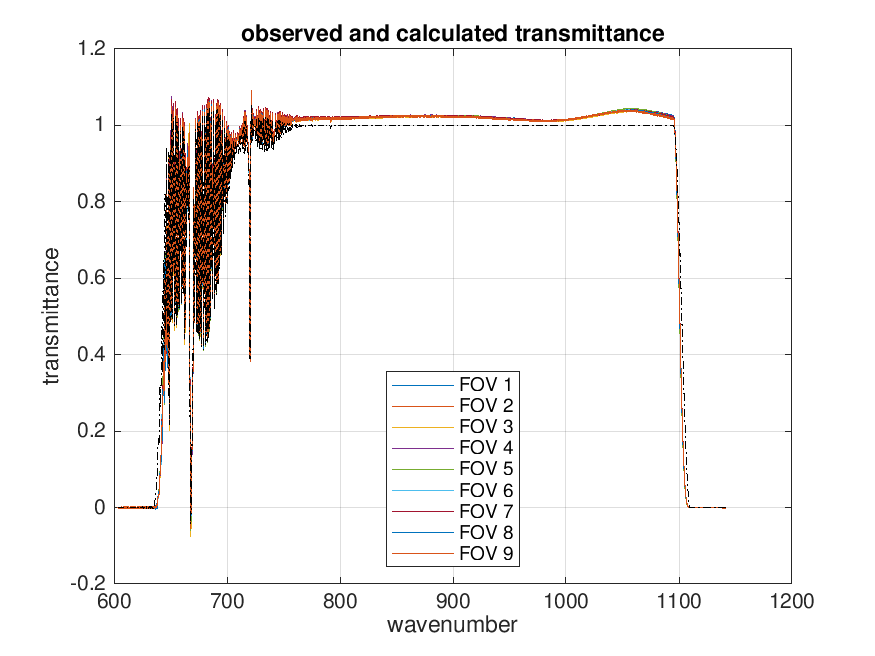
\includegraphics[width=\textwidth]{01-12_pfh_s1_CO2/spec_test2_all.png}
  \end{centering}\vspace{3mm}

Observed and calculated transmittance after the SA correction but
before any fitting. \\ We see a significant bias, possibly due to the
HTBB drifts.

\end{column}

\begin{column}{0.5\textwidth}
  \begin{centering}
  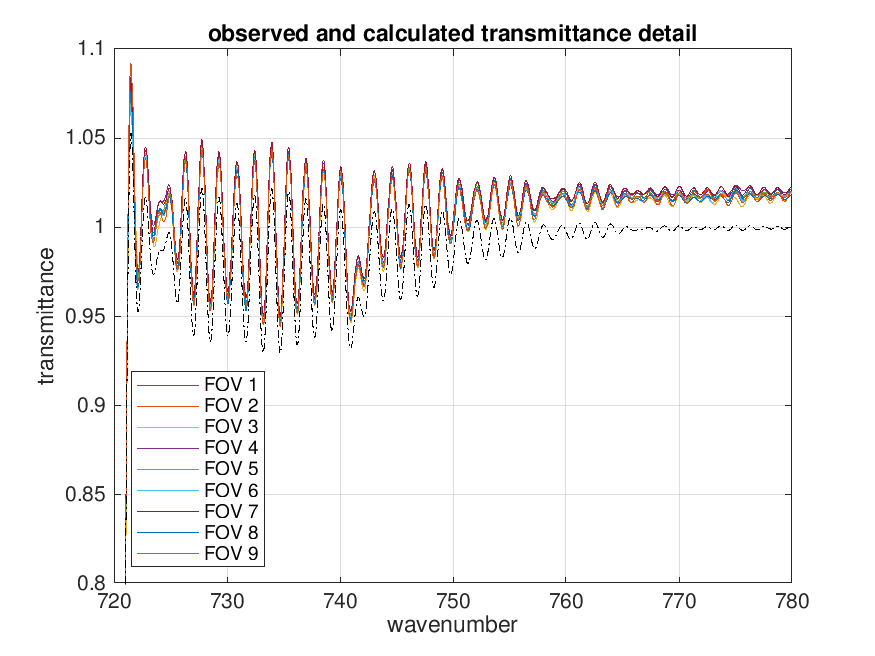
\includegraphics[width=\textwidth]{01-12_pfh_s1_CO2/spec_test2_zoom.png}
  \end{centering}\vspace{3mm}

A detail from the previous plot.  The FOV to FOV consistency is
relatively good.

\end{column}
\end{columns}
\end{frame}
%----------- slide --------------------------------------------------%
\begin{frame}
\frametitle{CO$_2$ side 1 fitting overview}
\begin{columns}[t]
\begin{column}{0.5\textwidth}  
  \begin{centering}
  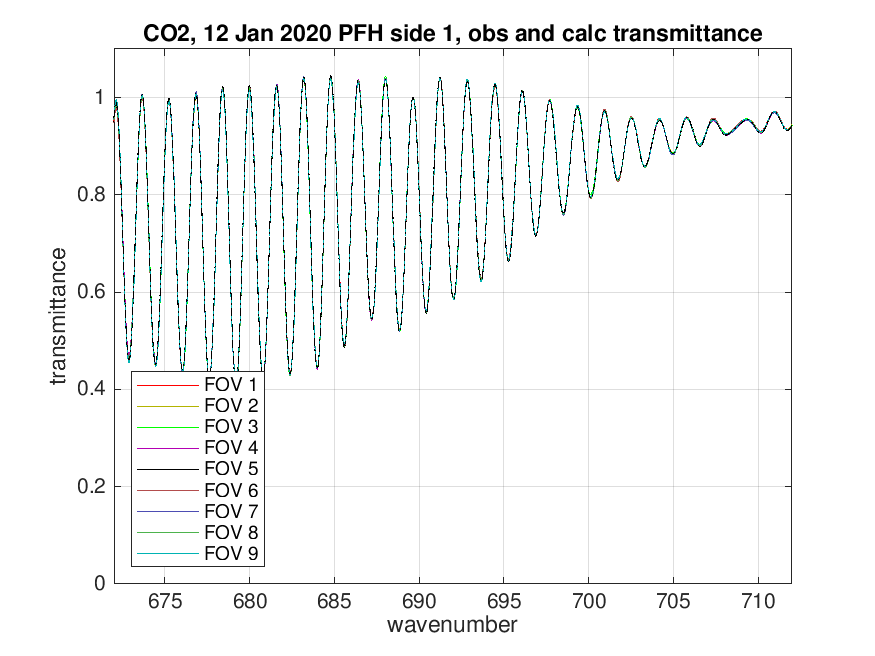
\includegraphics[width=\textwidth]{01-12_pfh_s1_CO2/CO2_obs_and_calc.png}
  \end{centering}\vspace{3mm}

Observed and calculated transmittance for all FOVs, over the fitting
interval.  At this level of detail we see all values are very close.

\end{column}

\begin{column}{0.5\textwidth}
  \begin{centering}
  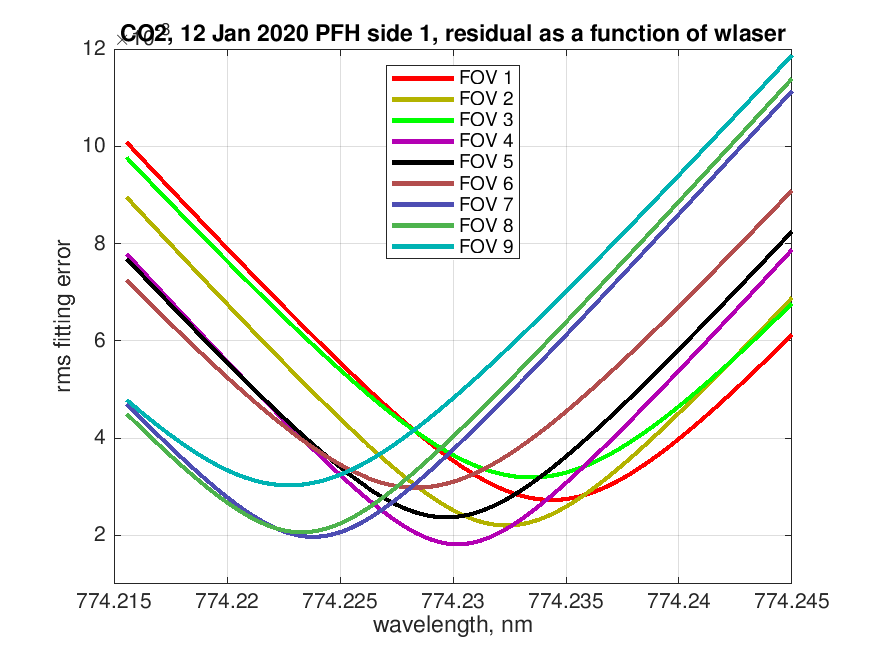
\includegraphics[width=\textwidth]{01-12_pfh_s1_CO2/CO2_wlaser_fit.png}
  \end{centering}\vspace{3mm}

Residuals $\rms(a\cdot\tauobs + b - \taucal)$ over the fitting
interval as a function of metrology laser wavelength, for each FOV.

\end{column}
\end{columns}
\end{frame}
%----------- slide --------------------------------------------------%
\begin{frame}
\frametitle{CO$_2$ side 1 obs minus calc breakouts}
\begin{columns}[t]
\begin{column}{0.5\textwidth}
  \begin{centering}
  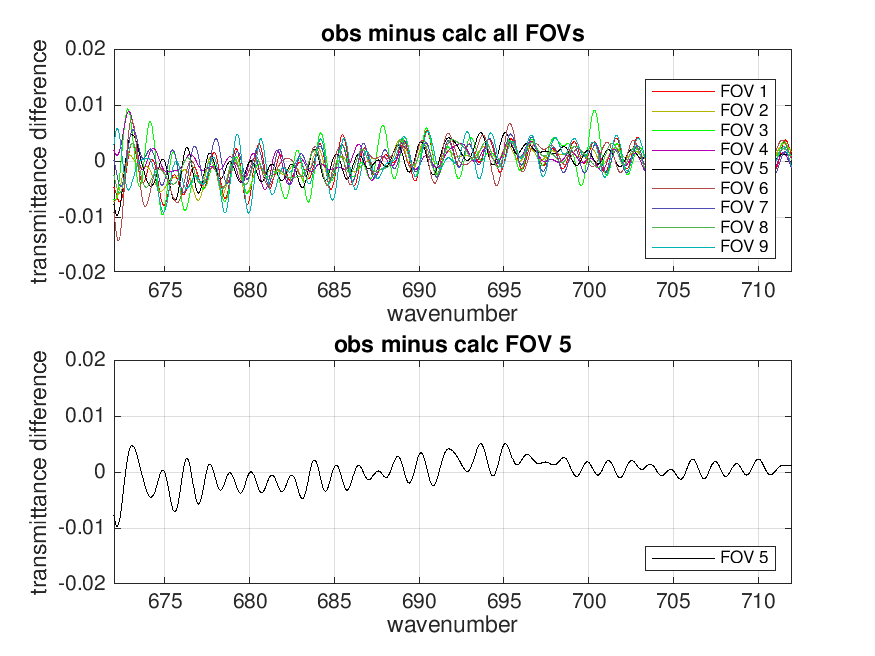
\includegraphics[width=\textwidth]{01-12_pfh_s1_CO2/CO2_breakout_1.png}
  \end{centering}\vspace{3mm}

Observed minus calculated transmittance for all FOVs and for FOV~5
alone, over the fitting interval.

\end{column}
\begin{column}{0.5\textwidth}  
  \begin{centering}
  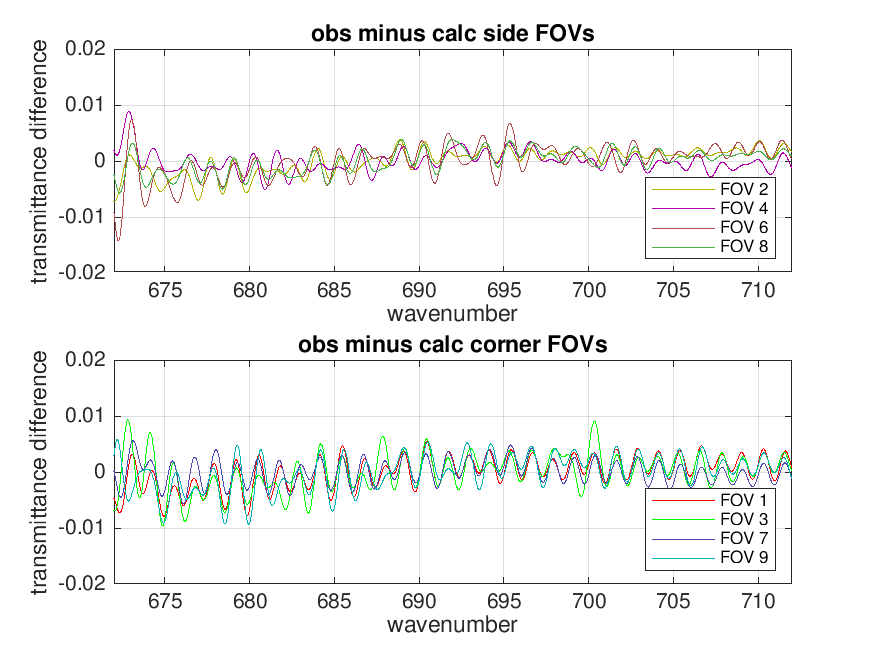
\includegraphics[width=\textwidth]{01-12_pfh_s1_CO2/CO2_breakout_2.png}
  \end{centering}\vspace{3mm}

Observed minus calculated transmittance for side and corner FOVs,
over the fitting interval.

\end{column}
\end{columns}
\end{frame}
%----------- slide --------------------------------------------------%
\begin{frame}[fragile]
\frametitle{CO$_2$ side 1 tabulated residuals}

  metrology laser absolute residuals, ppm
\begin{semiverbatim}\scriptsize
     -2.20     5.94    11.37         7   4   1
     -2.97     5.42     8.65         8   5   2
     -3.62     3.62    10.20         9   6   3
\end{semiverbatim}

  metrology laser relative residuals, ppm
\begin{semiverbatim}\scriptsize
     -7.62     0.52     5.94         7   4   1
     -8.40     0.00     3.23         8   5   2
     -9.04    -1.81     4.78         9   6   3
\end{semiverbatim}

     regression fitting weights and residuals
\begin{semiverbatim}\scriptsize
 FOV   "a"       "b"     dmin     wmin      wfov
  1   0.975    0.0032   0.0027    11.37   774.2344 
  2   0.975    0.0058   0.0022     8.65   774.2323 
  3   0.976    0.0060   0.0032    10.20   774.2335 
  4   0.968    0.0068   0.0018     5.94   774.2302 
  5   0.964    0.0144   0.0024     5.42   774.2298 
  6   0.982   -0.0013   0.0030     3.62   774.2284 
  7   0.976   -0.0037   0.0020    -2.20   774.2239 
  8   0.975    0.0052   0.0021    -2.97   774.2233 
  9   0.982   -0.0017   0.0030    -3.62   774.2228 
\end{semiverbatim}

\end{frame}
%----------- slide --------------------------------------------------%
\begin{frame}
\frametitle{CO$_2$ LW PFH side 2 test parameters}

\begin{itemize}
  \item PFH Plateau 21, 19 Jan 2019
  \item side 2, sweep direction 0
  \item fitting interval 672 to 712 $\wn$
  \item metrology laser 775.20773 nm, from neon 703.44765 nm
  \item ATBD default focal plane
  \item SA correction from ILS with periodic sinc at the sensor grid
  \item HTBB nominal T1 360 K, T2 320 K
  \item gas cell pressure 49.75 Torr
  \item gas cell temperature 17.27 C
  \item gas cell length 12.59 cm
\end{itemize}

\end{frame}
%----------- slide --------------------------------------------------%
\begin{frame}
\frametitle{CO$_2$ PFH side 2 cell empty test legs}
\begin{columns}[t]
\begin{column}{0.5\textwidth}
  \begin{centering}
  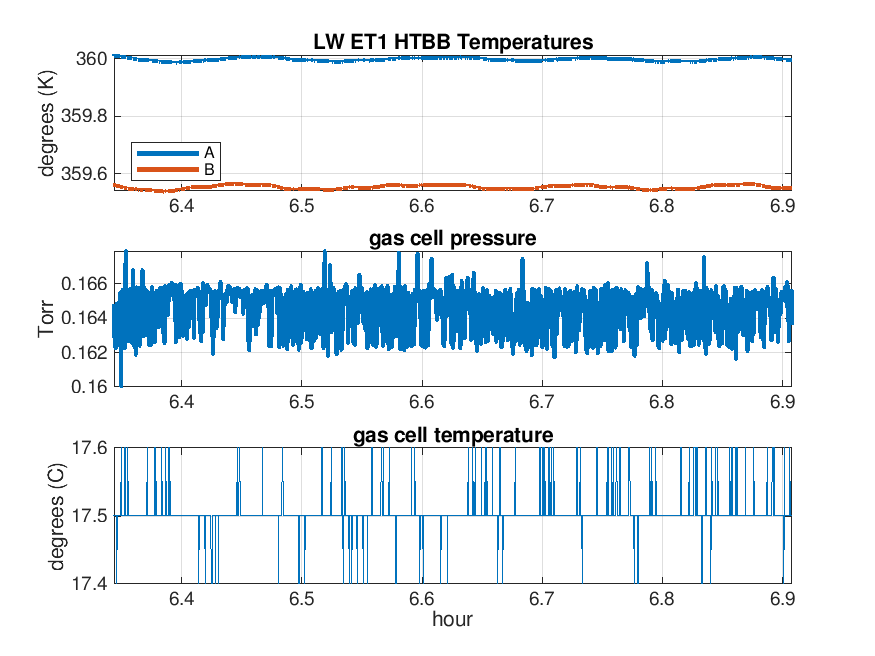
\includegraphics[width=\textwidth]{harvest_01-19/01-19_LW_ET1.png}
  \end{centering}\vspace{3mm}

  ET1 ``empty high'' leg of the the 19 Jan side 2 CO$_2$
  transmittance test.  The x-axis is hour of the day.  We see a
  small HTBB temperature wobble.

\end{column}
\begin{column}{0.5\textwidth}  
  \begin{centering}
  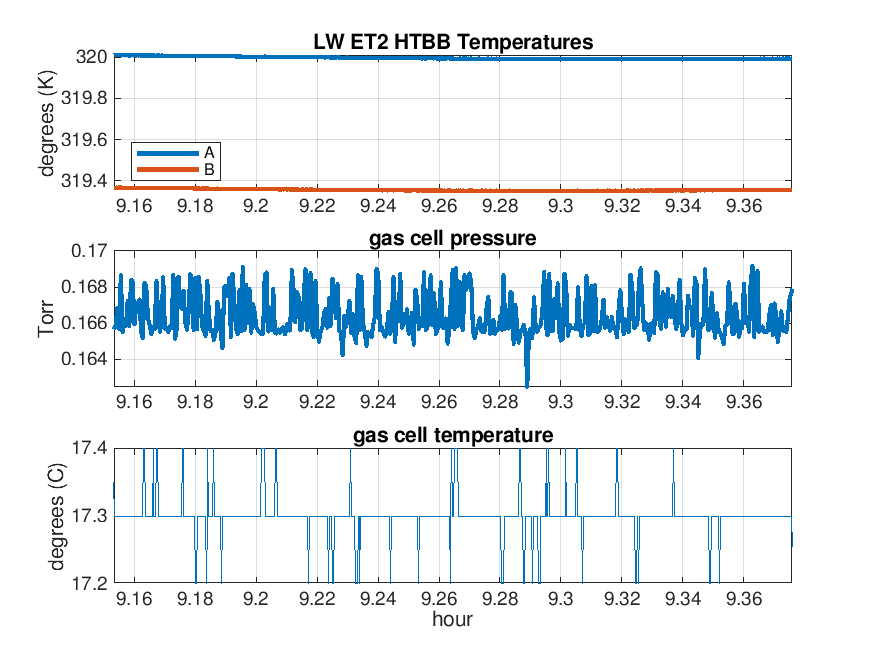
\includegraphics[width=\textwidth]{harvest_01-19/01-19_LW_ET2.png}
  \end{centering}\vspace{3mm}

  ET2 ``empty low'' leg of the the 13 Jan CO$_2$ transmittance test.
  This looks good.

\end{column}
\end{columns}
\end{frame}
%----------- slide --------------------------------------------------%
\begin{frame}
\frametitle{CO$_2$ PFH side 2 cell full test legs}
\begin{columns}[t]
\begin{column}{0.5\textwidth}
  \begin{centering}
  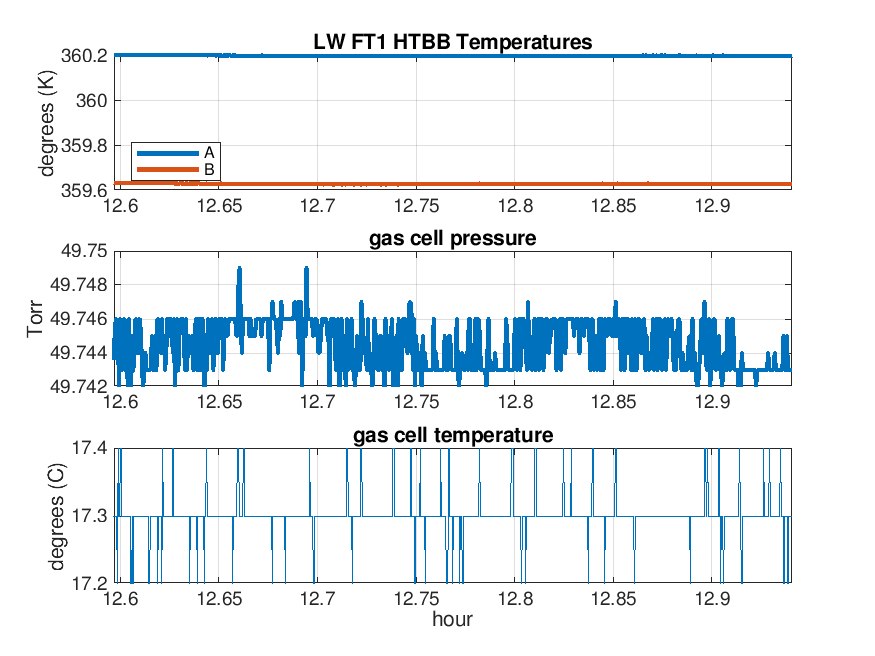
\includegraphics[width=\textwidth]{harvest_01-19/01-19_LW_FT1.png}
  \end{centering}\vspace{3mm}

  FT1 ``full high'' leg of the the 19 Jan CO$_2$ transmittance test.
  The x-axis is hour of the day.  This looks good

\end{column}
\begin{column}{0.5\textwidth}  
  \begin{centering}
  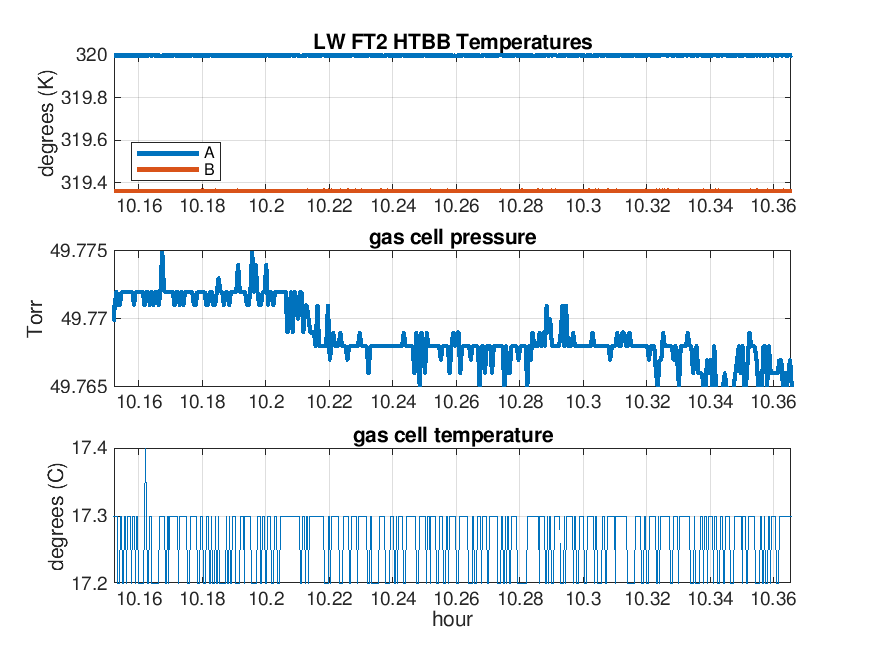
\includegraphics[width=\textwidth]{harvest_01-19/01-19_LW_FT2.png}
  \end{centering}\vspace{3mm}

  FT2 ``full low'' leg of the the 19 Jan CO$_2$ transmittance test.
  This looks good, the pressure drift is very small.

\end{column}
\end{columns}
\end{frame}
%----------- slide --------------------------------------------------%
\begin{frame}
\frametitle{CO$_2$ side 2 data before fitting}
\begin{columns}[t]
\begin{column}{0.5\textwidth}  
  \begin{centering}
  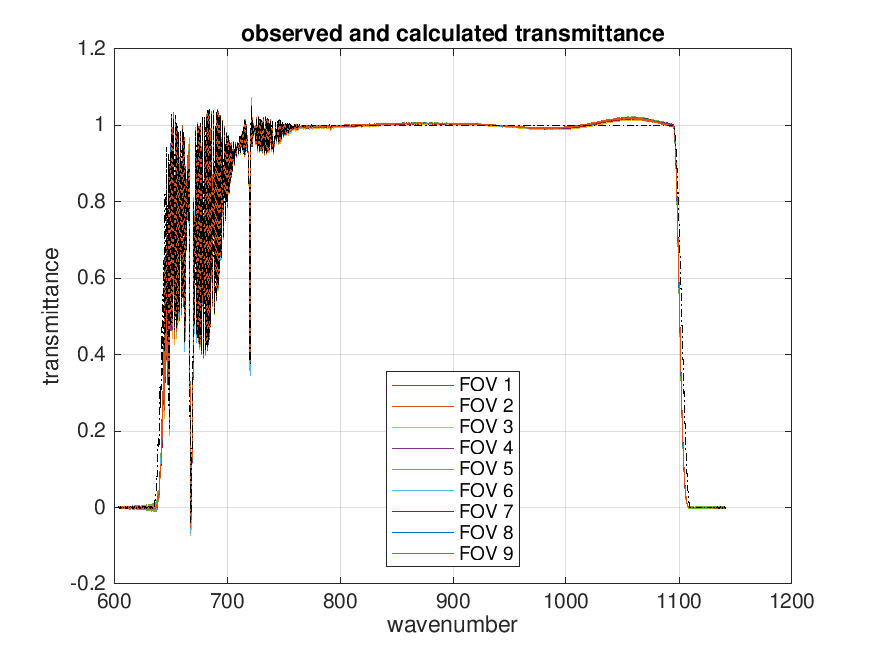
\includegraphics[width=\textwidth]{01-19_pfh_s2_CO2/spec_test2_all.png}
  \end{centering}\vspace{3mm}

Observed and calculated transmittance after the SA correction but
before any fitting.  This looks much better than the CO$_2$ side 1
case.

\end{column}

\begin{column}{0.5\textwidth}
  \begin{centering}
  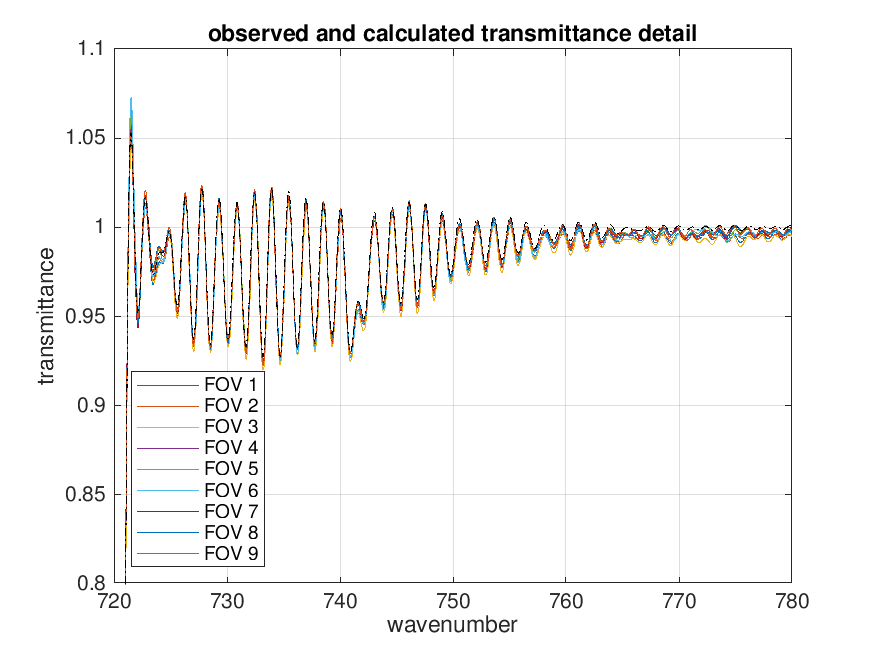
\includegraphics[width=\textwidth]{01-19_pfh_s2_CO2/spec_test2_zoom.png}
  \end{centering}\vspace{3mm}

A detail from the previous plot.  FOV to FOV consistency and
agreement with calculated transmittance is relatively good.

\end{column}
\end{columns}
\end{frame}
%----------- slide --------------------------------------------------%
\begin{frame}
\frametitle{CO$_2$ side 2 fitting overview}
\begin{columns}[t]
\begin{column}{0.5\textwidth}  
  \begin{centering}
  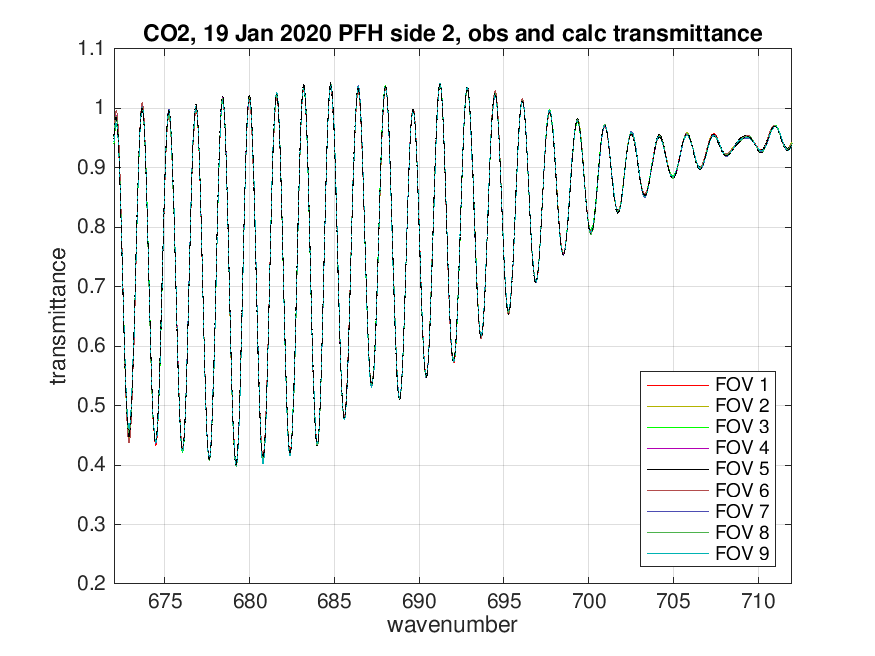
\includegraphics[width=\textwidth]{01-19_pfh_s2_CO2/CO2_obs_and_calc.png}
  \end{centering}\vspace{3mm}

Observed and calculated transmittance for all FOVs, over the fitting
interval.  At this level of detail we see all values are very close.

\end{column}

\begin{column}{0.5\textwidth}
  \begin{centering}
  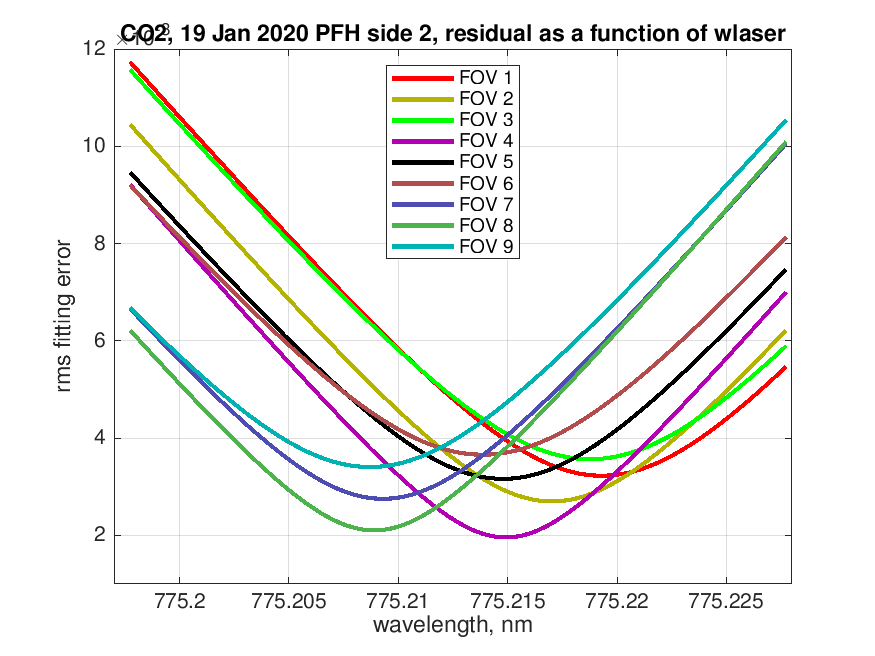
\includegraphics[width=\textwidth]{01-19_pfh_s2_CO2/CO2_wlaser_fit.png}
  \end{centering}\vspace{3mm}

Residuals $\rms(a\cdot\tauobs + b - \taucal)$ over the fitting
interval as a function of metrology laser wavelength, for each FOV.

\end{column}
\end{columns}
\end{frame}
%----------- slide --------------------------------------------------%
\begin{frame}
\frametitle{CO$_2$ side 2 obs minus calc breakouts}
\begin{columns}[t]
\begin{column}{0.5\textwidth}
  \begin{centering}
  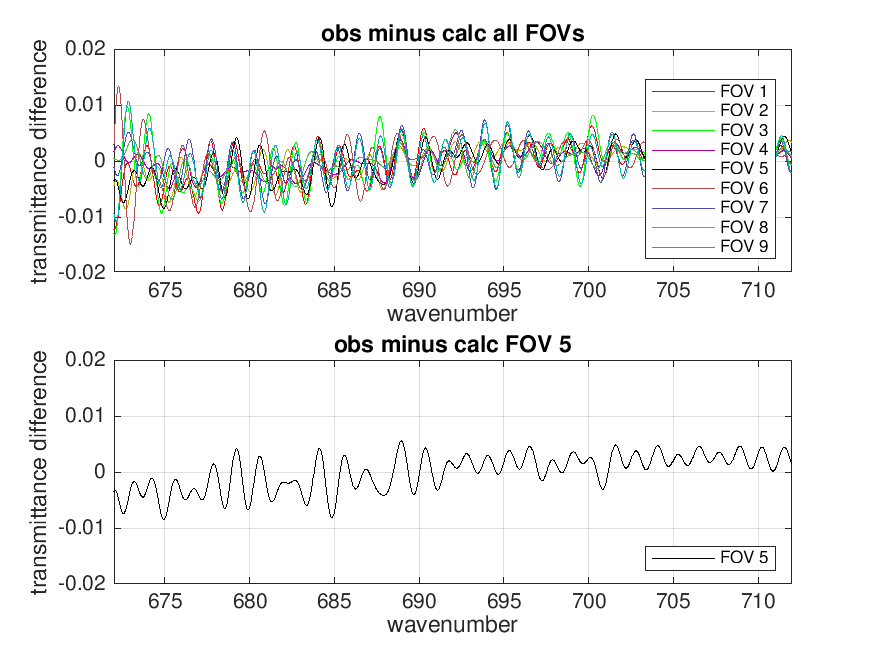
\includegraphics[width=\textwidth]{01-19_pfh_s2_CO2/CO2_breakout_1.png}
  \end{centering}\vspace{3mm}

Observed minus calculated transmittance for all FOVs and for FOV~5
alone, over the fitting interval.

\end{column}
\begin{column}{0.5\textwidth}  
  \begin{centering}
  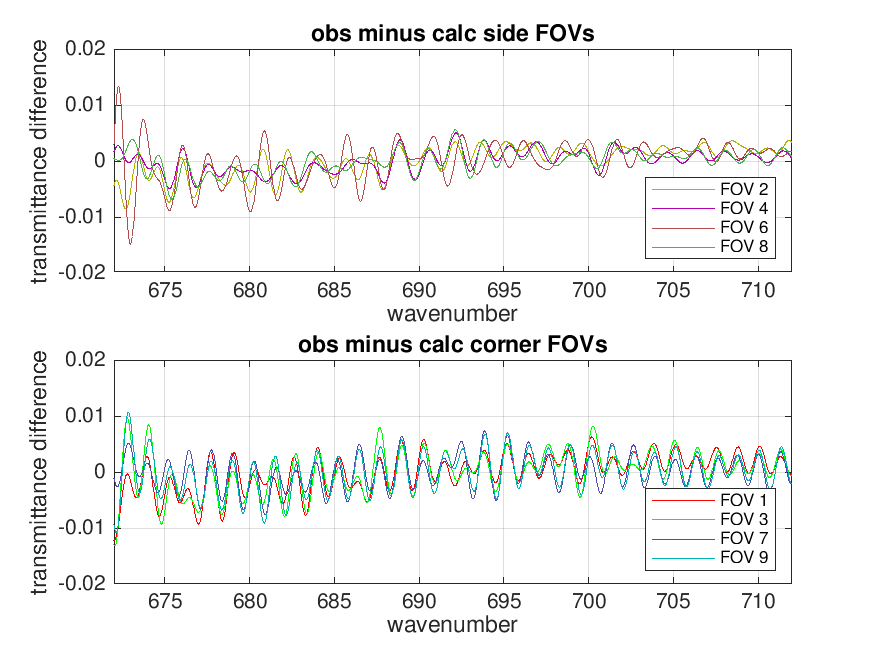
\includegraphics[width=\textwidth]{01-19_pfh_s2_CO2/CO2_breakout_2.png}
  \end{centering}\vspace{3mm}

Observed minus calculated transmittance for side and corner FOVs,
over the fitting interval.

\end{column}
\end{columns}
\end{frame}
%----------- slide --------------------------------------------------%
\begin{frame}[fragile]
\frametitle{CO$_2$ side 2 tabulated residuals}

  metrology laser absolute residuals, ppm
\begin{semiverbatim}\scriptsize
      2.06     9.29    14.96         7   4   1
      1.55     9.16    12.00         8   5   2
      1.16     8.00    14.32         9   6   3
\end{semiverbatim}

  metrology laser relative residuals, ppm
\begin{semiverbatim}\scriptsize
     -7.09     0.13     5.80         7   4   1
     -7.61     0.00     2.84         8   5   2
     -8.00    -1.16     5.16         9   6   3
\end{semiverbatim}

     regression fitting weights and residuals
\begin{semiverbatim}\scriptsize
 FOV   "a"       "b"     dmin     wmin      wfov
  1   0.996    0.0071   0.0032    14.96   775.2193 
  2   0.995    0.0095   0.0027    12.00   775.2170 
  3   0.997    0.0084   0.0036    14.32   775.2188 
  4   0.989    0.0105   0.0020     9.29   775.2149 
  5   0.997    0.0045   0.0032     9.16   775.2148 
  6   0.996    0.0062   0.0037     8.00   775.2139 
  7   0.994    0.0059   0.0028     2.06   775.2093 
  8   0.994    0.0052   0.0021     1.55   775.2089 
  9   0.995    0.0041   0.0034     1.16   775.2086 
\end{semiverbatim}

\end{frame}
%----------- slide --------------------------------------------------%
\begin{frame}
\frametitle{CH$_4$ MW PFH side 1 test parameters}

\begin{itemize}
  \item PFH Plateau 21, 13 Jan 2019
  \item side 1, sweep direction 0
  \item fitting interval 1220 to 1380 $\wn$
  \item metrology laser 774.22465 nm, from neon 703.44765 nm
  \item ATBD default focal plane
  \item SA correction from ILS with periodic sinc at the sensor grid
  \item HTBB nominal T1 360 K, T2 320 K
  \item gas cell pressure 48.70 Torr
  \item gas cell temperature 17.17 C
  \item gas cell length 12.59 cm
\end{itemize}

\end{frame}
%----------- slide --------------------------------------------------%
\begin{frame}
\frametitle{CH$_4$ PFH side 1 cell empty test legs}
\begin{columns}[t]
\begin{column}{0.5\textwidth}
  \begin{centering}
  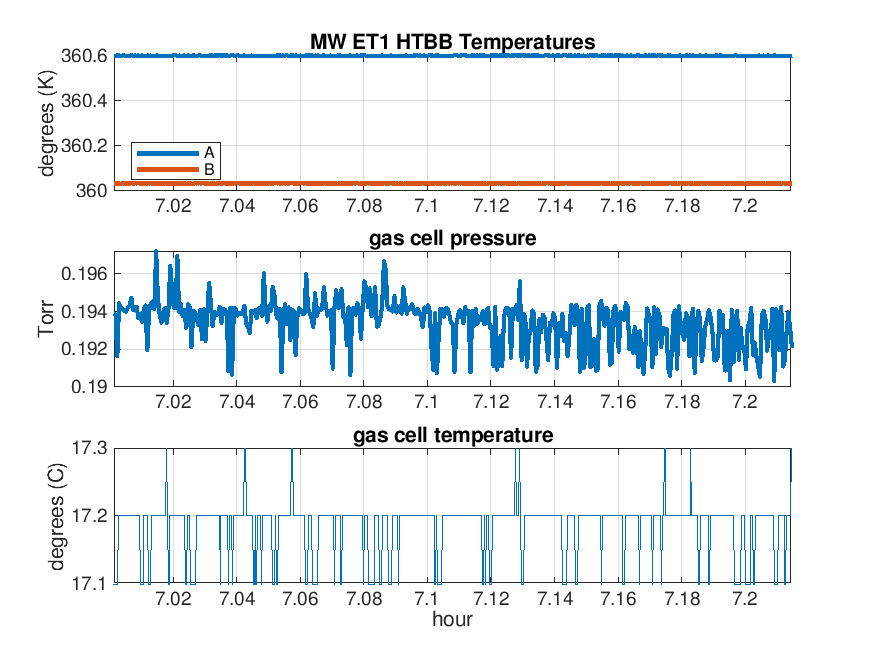
\includegraphics[width=\textwidth]{harvest_01-12/01-13_MW_ET1.png}
  \end{centering}\vspace{3mm}

  ET1 ``empty high'' leg of the the 13 Jan CH$_4$ transmittance test.
  The x-axis is hour of the day.  This looks good.

\end{column}
\begin{column}{0.5\textwidth}  
  \begin{centering}
  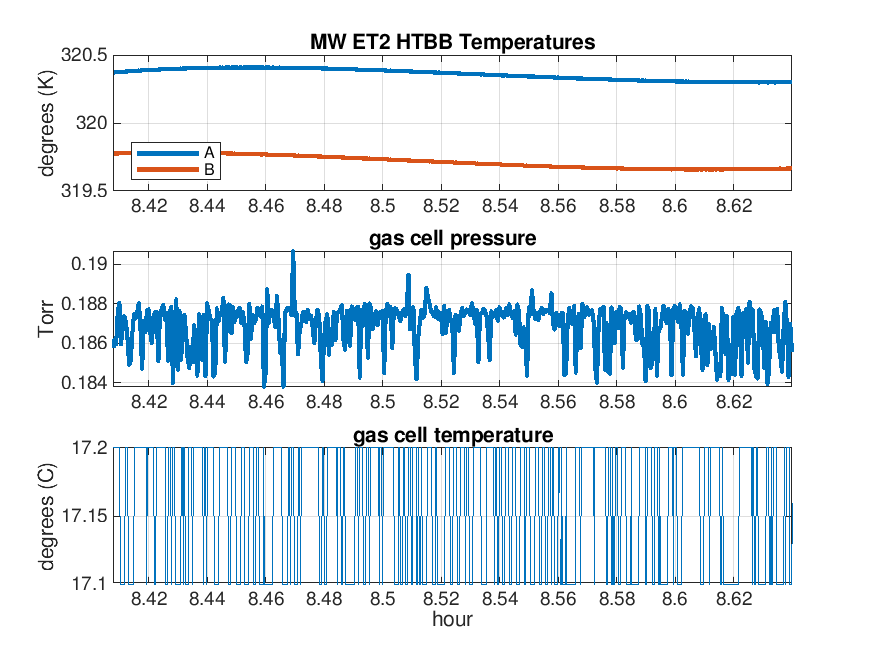
\includegraphics[width=\textwidth]{harvest_01-12/01-13_MW_ET2.png}
  \end{centering}\vspace{3mm}

  ET2 ``empty low'' leg of the the 13 Jan CH$_4$ transmittance test.
  We see some HTBB drift.

\end{column}
\end{columns}
\end{frame}
%----------- slide --------------------------------------------------%
\begin{frame}
\frametitle{CH$_4$ PFH side 1 cell full test legs}
\begin{columns}[t]
\begin{column}{0.5\textwidth}
  \begin{centering}
  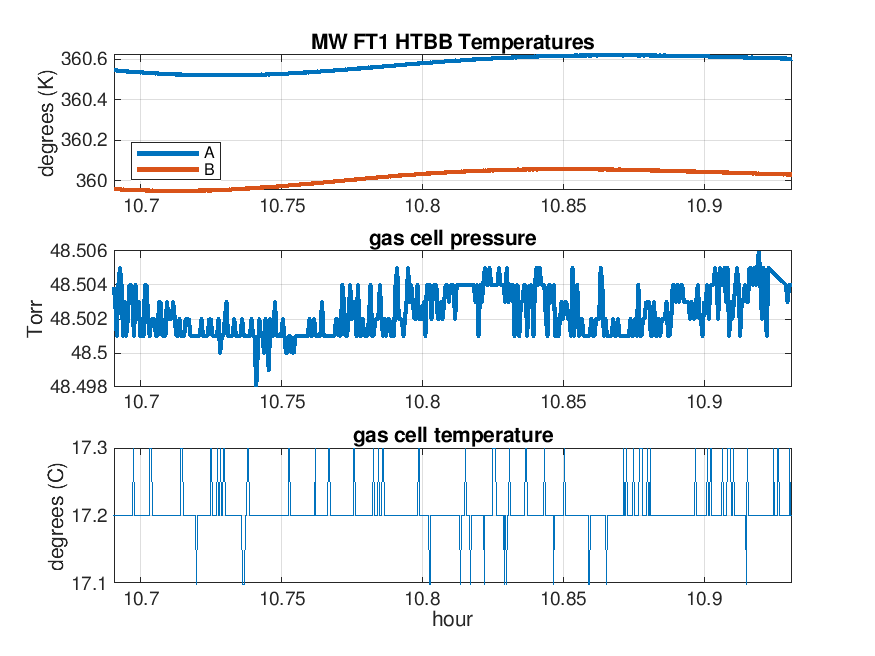
\includegraphics[width=\textwidth]{harvest_01-12/01-13_MW_FT1.png}
  \end{centering}\vspace{3mm}

  FT1 ``full high'' leg of the the 13 Jan CH$_4$ transmittance test.
  The x-axis is hour of the day.  As in the empty low leg we see
  some HTBB drift.

\end{column}
\begin{column}{0.5\textwidth}  
  \begin{centering}
  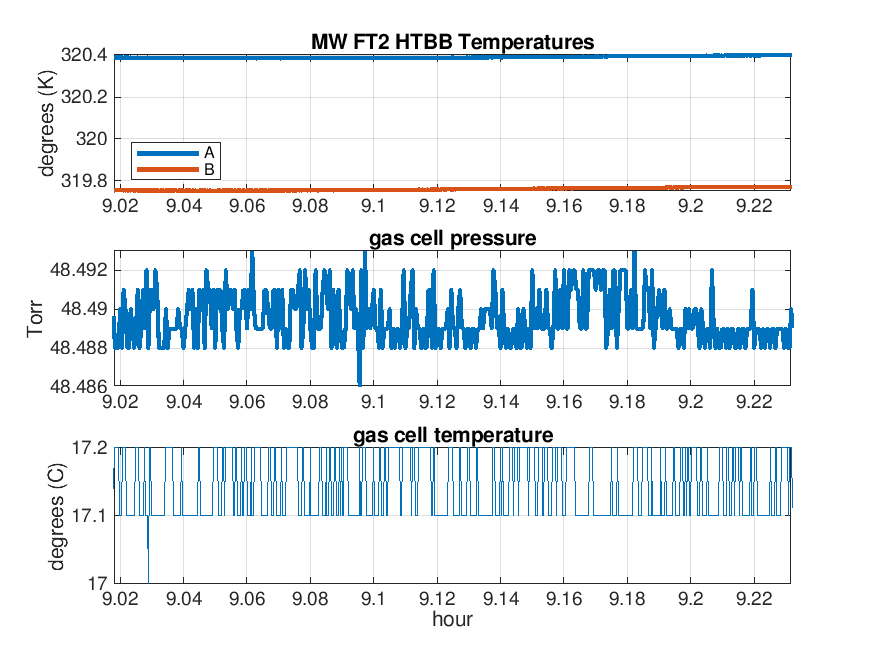
\includegraphics[width=\textwidth]{harvest_01-12/01-13_MW_FT2.png}
  \end{centering}\vspace{3mm}

  FT2 ``full low'' leg of the the 13 Jan CH$_4$ transmittance test.
  This looks good.

\end{column}
\end{columns}
\end{frame}
%----------- slide --------------------------------------------------%
\begin{frame}
\frametitle{CH$_4$ side 1 data before fitting}
\begin{columns}[t]
\begin{column}{0.5\textwidth}  
  \begin{centering}
  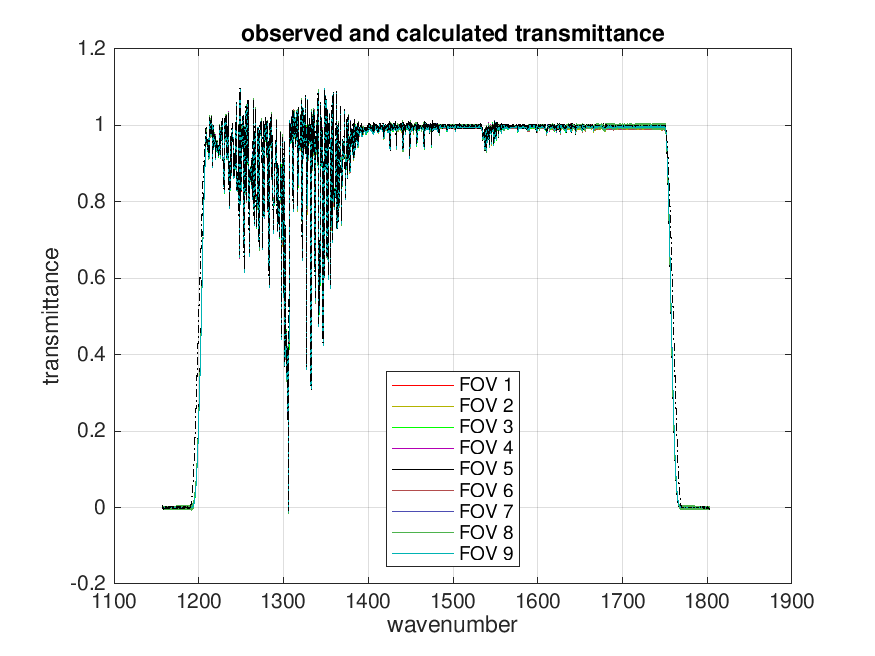
\includegraphics[width=\textwidth]{01-13_pfh_s1_CH4/spec_test2_all.png}
  \end{centering}\vspace{3mm}

Observed and calculated transmittance after the SA correction but
before fitting.  \\ This looks relatively good

\end{column}

\begin{column}{0.5\textwidth}
  \begin{centering}
  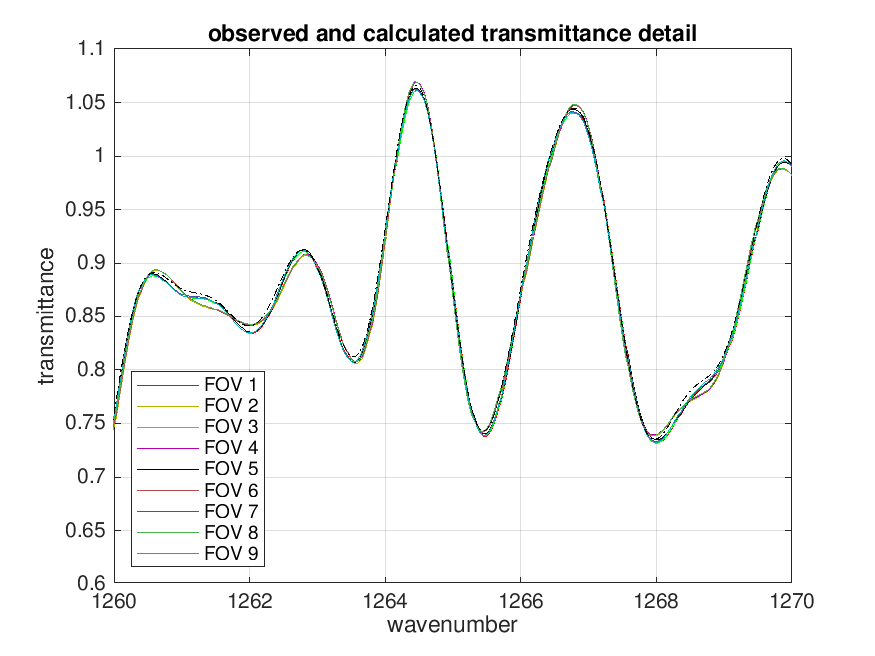
\includegraphics[width=\textwidth]{01-13_pfh_s1_CH4/spec_test2_zoom.png}
  \end{centering}\vspace{3mm}

A detail from the previous plot. \\ The FOV to FOV consistency and
bias are of a similar, relatively small magnitude.

\end{column}
\end{columns}
\end{frame}
%----------- slide --------------------------------------------------%
\begin{frame}
\frametitle{CH$_4$ side 1 fitting overview}
\begin{columns}[t]
\begin{column}{0.5\textwidth}  
  \begin{centering}
  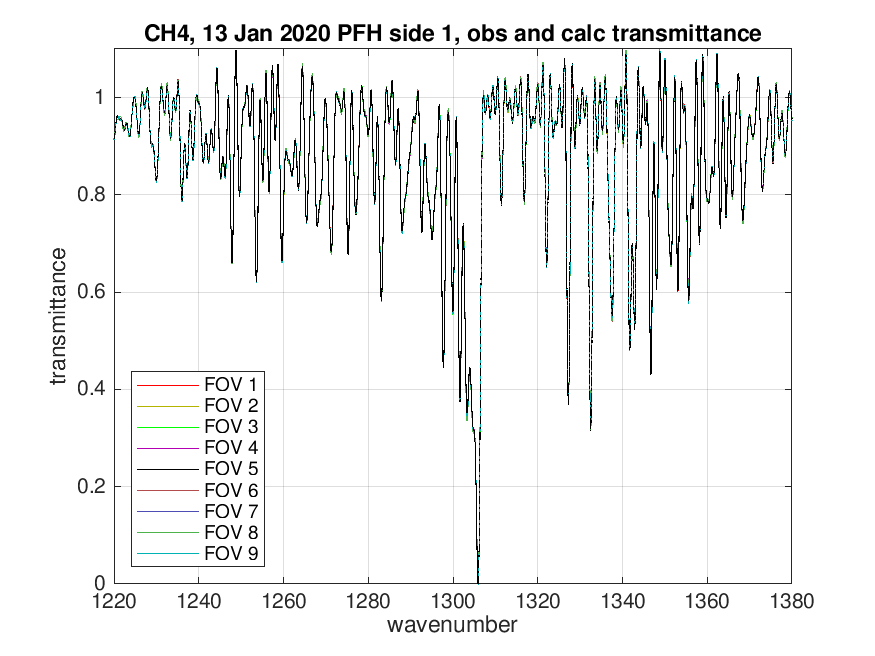
\includegraphics[width=\textwidth]{01-13_pfh_s1_CH4/CH4_obs_and_calc.png}
  \end{centering}\vspace{3mm}

Observed and calculated transmittance for all FOVs, over the fitting
interval.  At this level of detail we see all values are very close.

\end{column}

\begin{column}{0.5\textwidth}
  \begin{centering}
  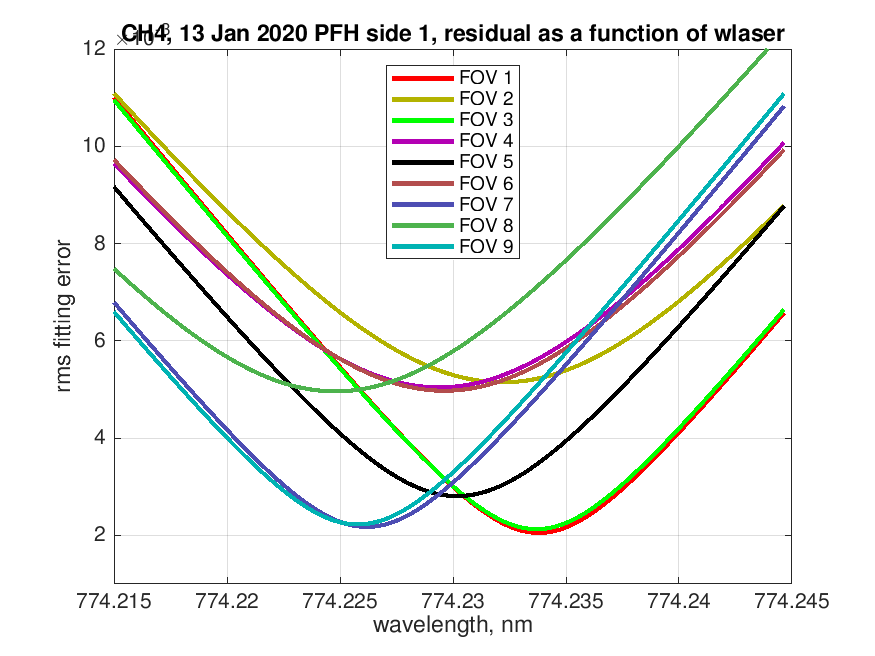
\includegraphics[width=\textwidth]{01-13_pfh_s1_CH4/CH4_wlaser_fit.png}
  \end{centering}\vspace{3mm}

Residuals $\rms(a\cdot\tauobs + b - \taucal)$ over the fitting
interval as a function of metrology laser wavelength, for each FOV.

\end{column}
\end{columns}
\end{frame}
%----------- slide --------------------------------------------------%
\begin{frame}
\frametitle{CH$_4$ side 1 obs minus calc breakouts}
\begin{columns}[t]
\begin{column}{0.5\textwidth}
  \begin{centering}
  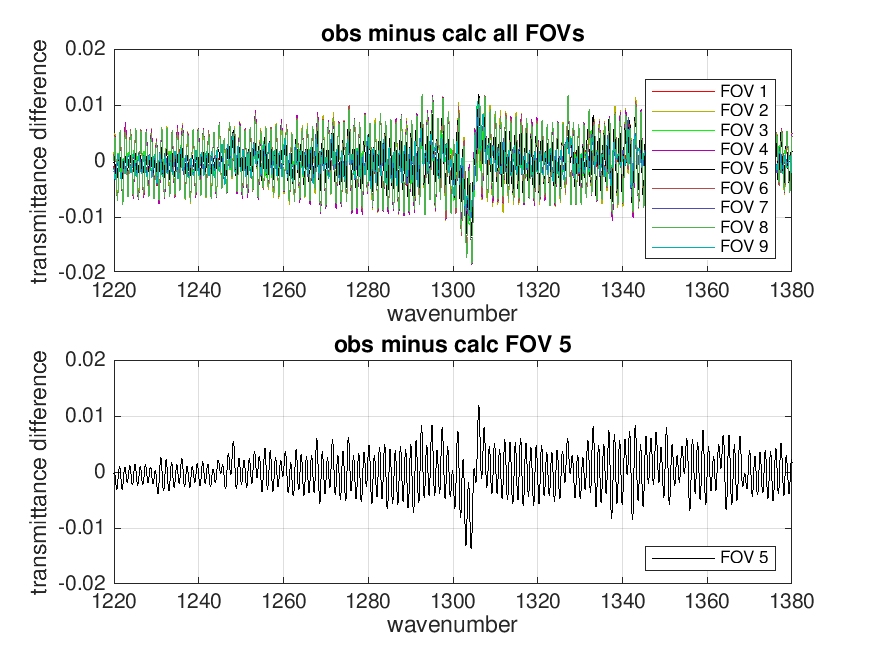
\includegraphics[width=\textwidth]{01-13_pfh_s1_CH4/CH4_breakout_1.png}
  \end{centering}\vspace{3mm}

Observed minus calculated transmittance for all FOVs and for FOV~5
alone, over the fitting interval.

\end{column}
\begin{column}{0.5\textwidth}  
  \begin{centering}
  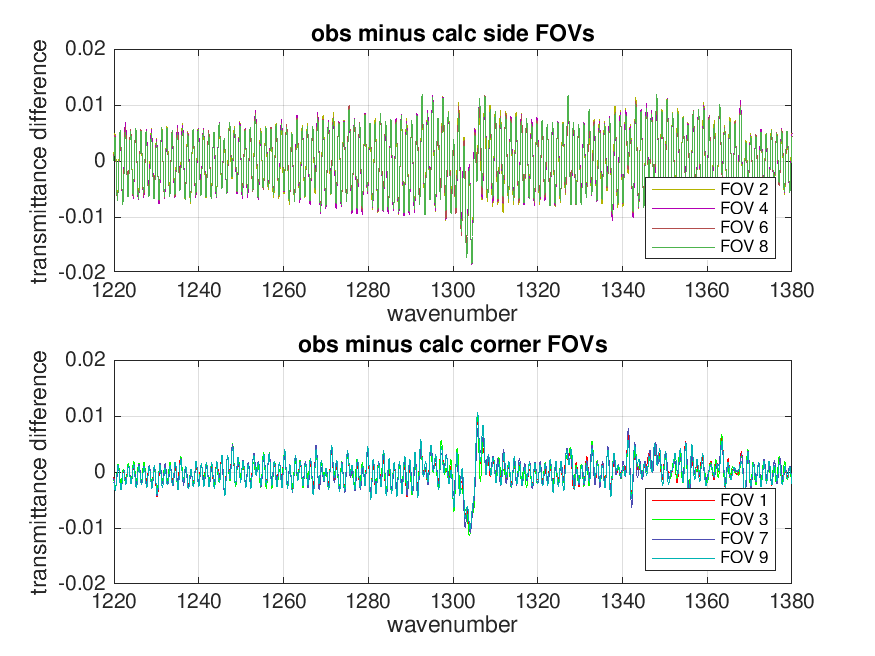
\includegraphics[width=\textwidth]{01-13_pfh_s1_CH4/CH4_breakout_2.png}
  \end{centering}\vspace{3mm}

Observed minus calculated transmittance for side and corner FOVs,
over the fitting interval.

\end{column}
\end{columns}
\end{frame}
%----------- slide --------------------------------------------------%
\begin{frame}[fragile]
\frametitle{CH$_4$ side 1 tabulated residuals}

  metrology laser absolute residuals, ppm
\begin{semiverbatim}\scriptsize
      1.94     6.07    11.75         7   4   1
      0.26     7.23     9.69         8   5   2
      1.42     6.46    11.62         9   6   3
\end{semiverbatim}

  metrology laser relative residuals, ppm
\begin{semiverbatim}\scriptsize
     -5.30    -1.16     4.52         7   4   1
     -6.97     0.00     2.45         8   5   2
     -5.81    -0.77     4.39         9   6   3
 \end{semiverbatim}

     regression fitting weights and residuals
\begin{semiverbatim}\scriptsize
 FOV   "a"       "b"     dmin     wmin      wfov
  1   0.991    0.0122   0.0020    11.75   774.2338 
  2   0.994    0.0087   0.0051     9.69   774.2322 
  3   0.992    0.0108   0.0021    11.62   774.2337 
  4   0.994    0.0080   0.0050     6.07   774.2294 
  5   0.992    0.0101   0.0028     7.23   774.2303 
  6   0.995    0.0073   0.0050     6.46   774.2297 
  7   0.992    0.0096   0.0022     1.94   774.2262 
  8   0.995    0.0071   0.0050     0.26   774.2249 
  9   0.992    0.0103   0.0022     1.42   774.2258 
\end{semiverbatim}

\end{frame}
%----------- slide --------------------------------------------------%
\begin{frame}
\frametitle{CO SW PFH side 1 test parameters}

\begin{itemize}
  \item PFH Plateau 21, 13 Jan 2019
  \item side 1, sweep direction 0
  \item fitting interval 2160 to 2240 $\wn$
  \item metrology laser 774.22453 nm, from neon 703.44765 nm
  \item ATBD default focal plane
  \item SA correction from ILS with periodic sinc at the sensor grid
  \item HTBB nominal T1 335 K, T2 320 K
  \item gas cell pressure 49.58 Torr
  \item gas cell temperature 17.15 C
  \item gas cell length 12.59 cm
\end{itemize}

\end{frame}
%----------- slide --------------------------------------------------%
\begin{frame}
\frametitle{CO PFH side 1 cell empty test legs}
\begin{columns}[t]
\begin{column}{0.5\textwidth}
  \begin{centering}
  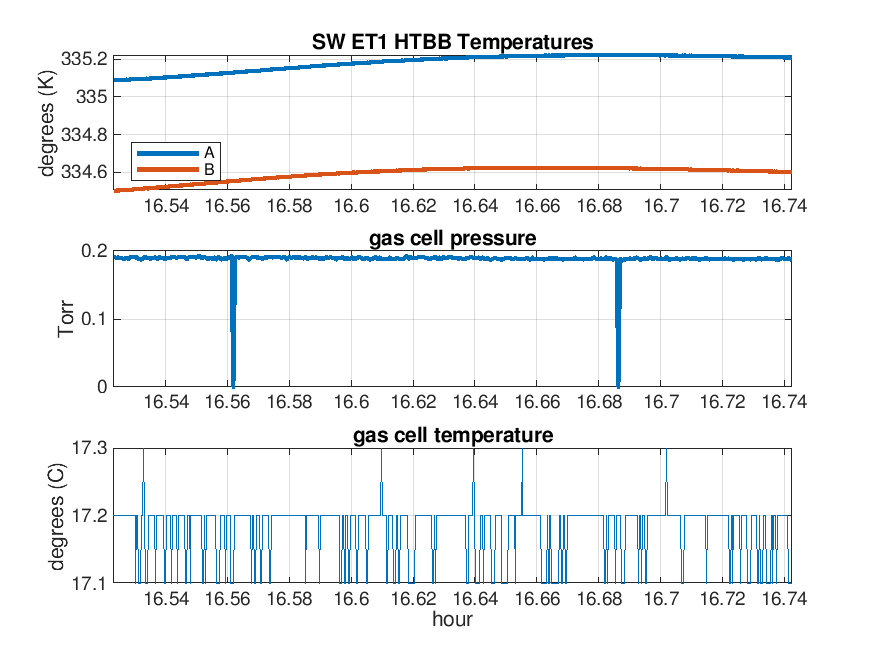
\includegraphics[width=\textwidth]{harvest_01-12/01-13_SW_ET1.png}
  \end{centering}\vspace{3mm}

  ET1 ``empty high'' leg of the the 13 Jan CO transmittance test.
  The x-axis here is hour of the day.  We see some HTBB drift.

\end{column}
\begin{column}{0.5\textwidth}  
  \begin{centering}
  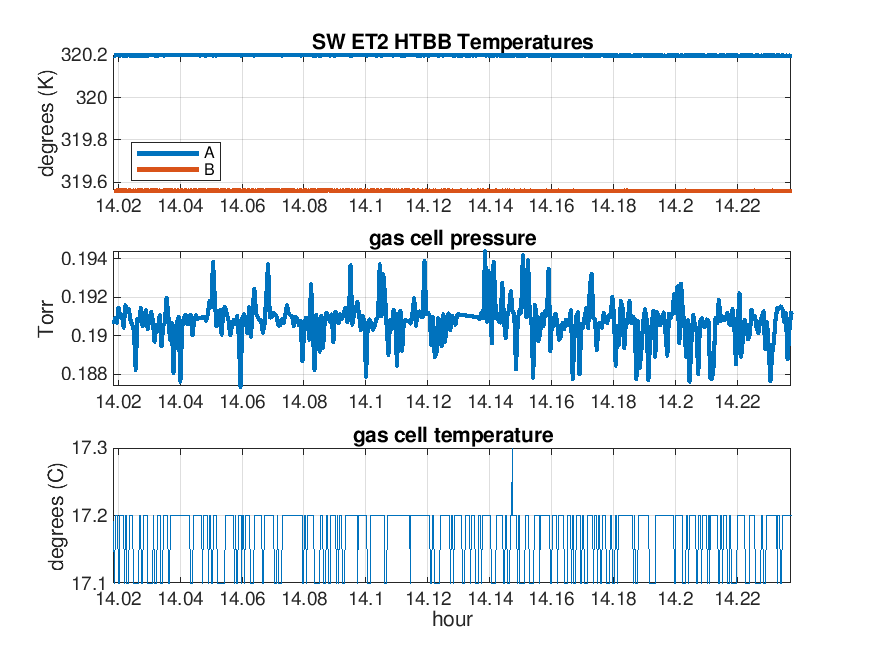
\includegraphics[width=\textwidth]{harvest_01-12/01-13_SW_ET2.png}
  \end{centering}\vspace{3mm}

  ET2 ``empty low'' leg of the the 13 Jan CO transmittance test.
  This looks good.  

\end{column}
\end{columns}
\end{frame}
%----------- slide --------------------------------------------------%
\begin{frame}
\frametitle{CO PFH side 1 cell full test legs}
\begin{columns}[t]
\begin{column}{0.5\textwidth}
  \begin{centering}
  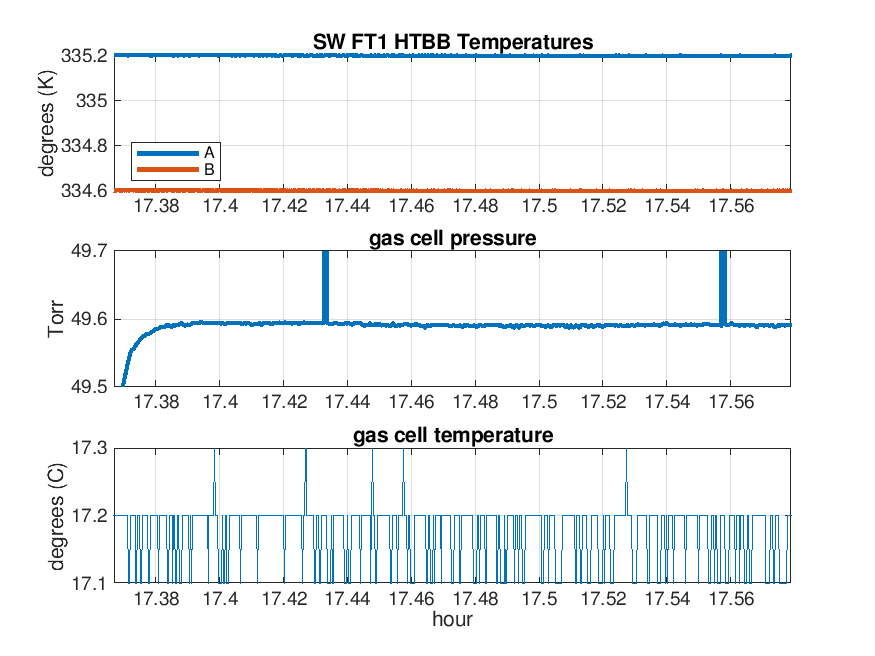
\includegraphics[width=\textwidth]{harvest_01-12/01-13_SW_FT1.png}
  \end{centering}\vspace{3mm}

  FT1 ``full high'' leg of the the 13 Jan CO transmittance test.
  HTBB temps look good but we have a small droop in pressure at the
  start.

\end{column}
\begin{column}{0.5\textwidth}  
  \begin{centering}
  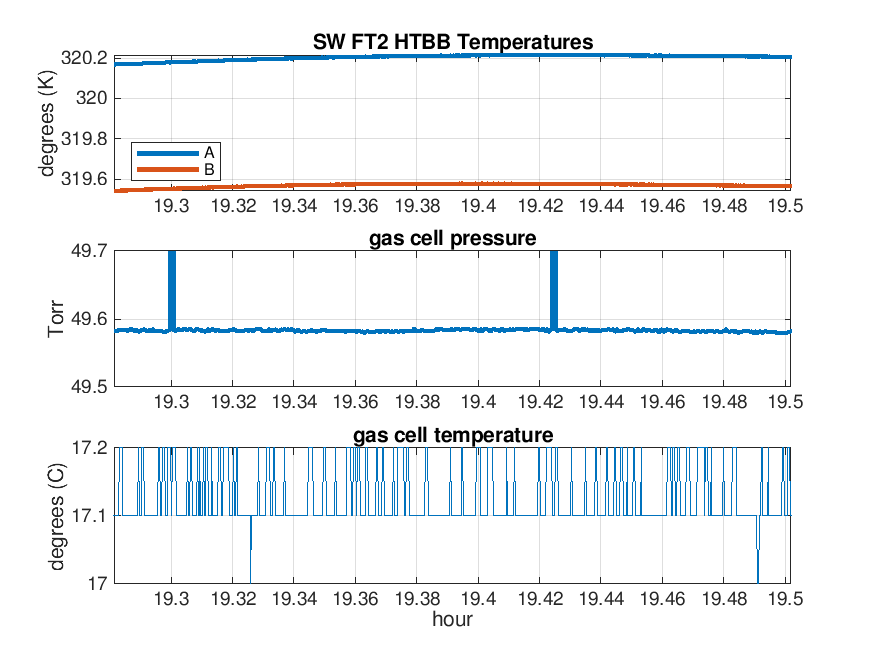
\includegraphics[width=\textwidth]{harvest_01-12/01-13_SW_FT2.png}
  \end{centering}\vspace{3mm}

  FT2 ``full low'' leg of the the 13 Jan CO transmittance test.
  There is a small HTBB drift.

\end{column}
\end{columns}
\end{frame}
%----------- slide --------------------------------------------------%
\begin{frame}
\frametitle{CO side 1 data before fitting}
\begin{columns}[t]
\begin{column}{0.5\textwidth}  
  \begin{centering}
  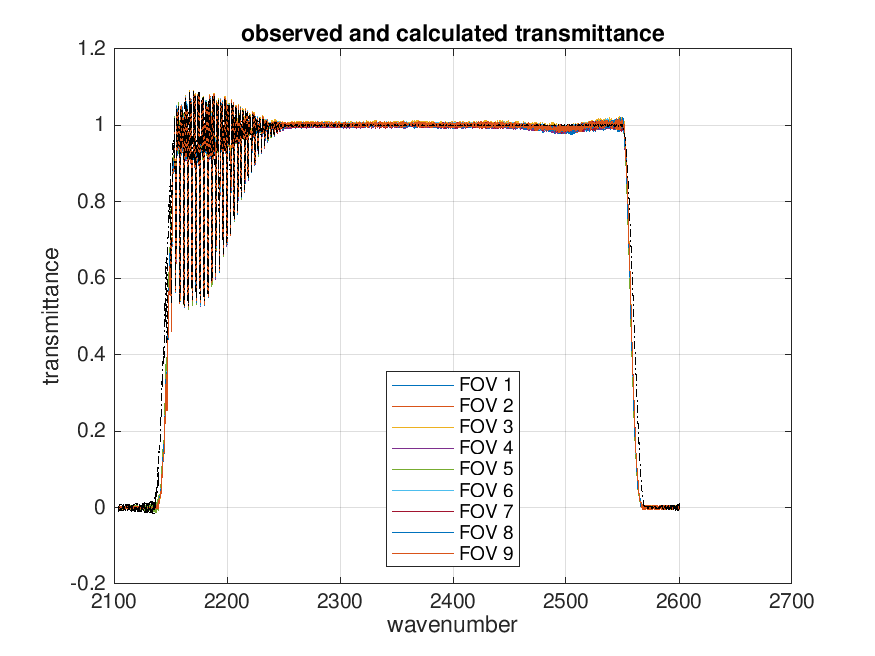
\includegraphics[width=\textwidth]{01-13_pfh_s1_CO/spec_test2_all.png}
  \end{centering}\vspace{3mm}

Observed and calculated transmittance after the SA correction but
before fitting. \\ This looks relatively good.

\end{column}

\begin{column}{0.5\textwidth}
  \begin{centering}
  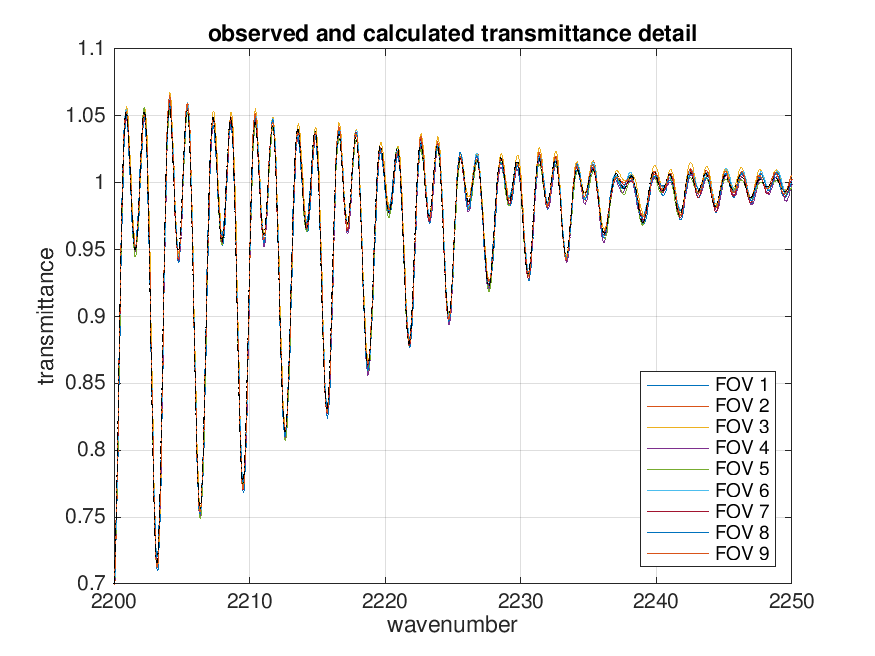
\includegraphics[width=\textwidth]{01-13_pfh_s1_CO/spec_test2_zoom.png}
  \end{centering}\vspace{3mm}

A detail from the previous plot.  This looks good.

\end{column}
\end{columns}
\end{frame}
%----------- slide --------------------------------------------------%
\begin{frame}
\frametitle{CO side 1 fitting overview}
\begin{columns}[t]
\begin{column}{0.5\textwidth}  
  \begin{centering}
  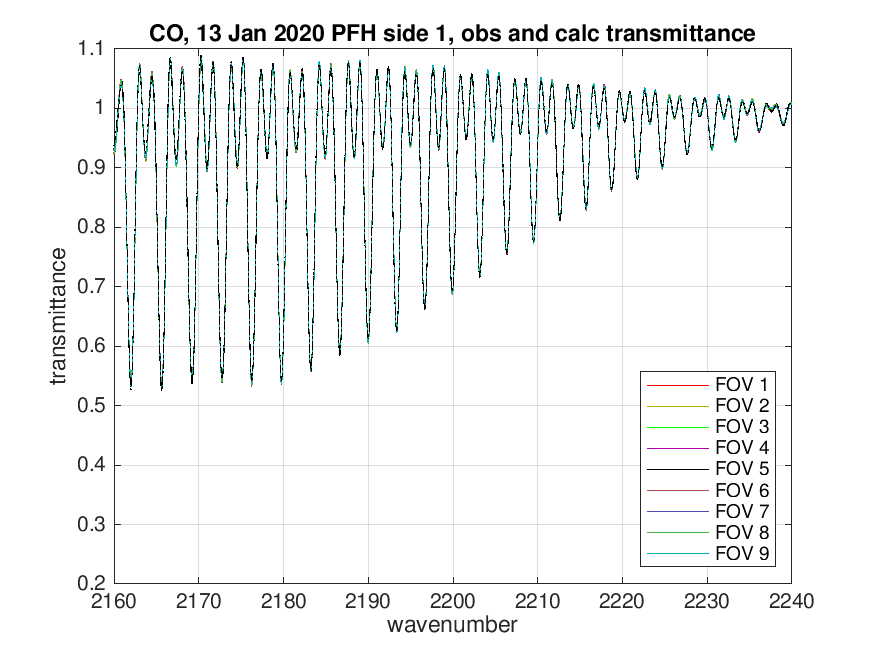
\includegraphics[width=\textwidth]{01-13_pfh_s1_CO/CO_obs_and_calc.png}
  \end{centering}\vspace{3mm}

Observed and calculated transmittance for all FOVs, over the fitting
interval.  At this level of detail we see all values are very close.

\end{column}

\begin{column}{0.5\textwidth}
  \begin{centering}
  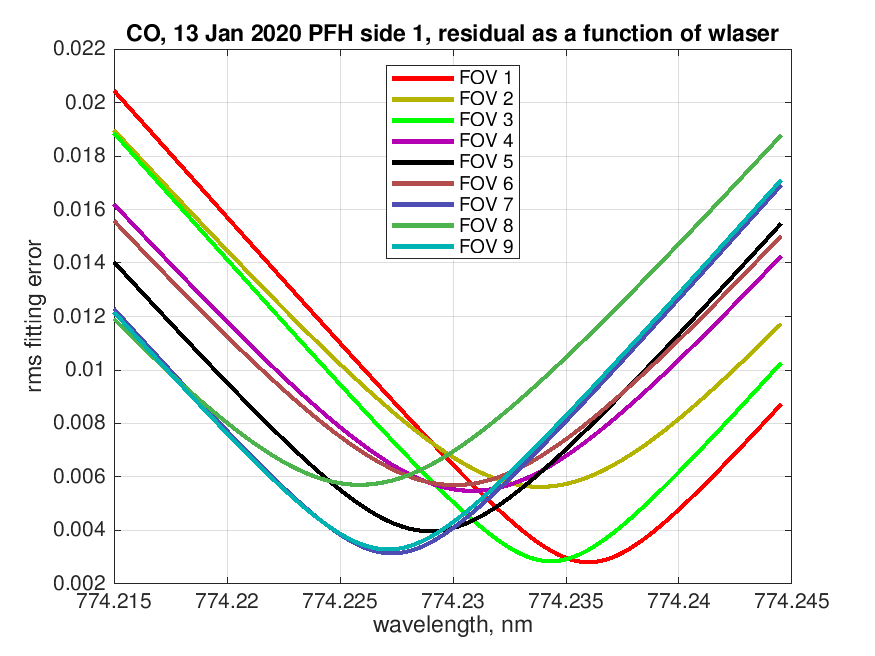
\includegraphics[width=\textwidth]{01-13_pfh_s1_CO/CO_wlaser_fit.png}
  \end{centering}\vspace{3mm}

Residuals $\rms(a\cdot\tauobs + b - \taucal)$ over the fitting
interval as a function of metrology laser wavelength, for each FOV.

\end{column}
\end{columns}
\end{frame}
%----------- slide --------------------------------------------------%
\begin{frame}
\frametitle{CO side 1 obs minus calc breakouts}
\begin{columns}[t]
\begin{column}{0.5\textwidth}
  \begin{centering}
  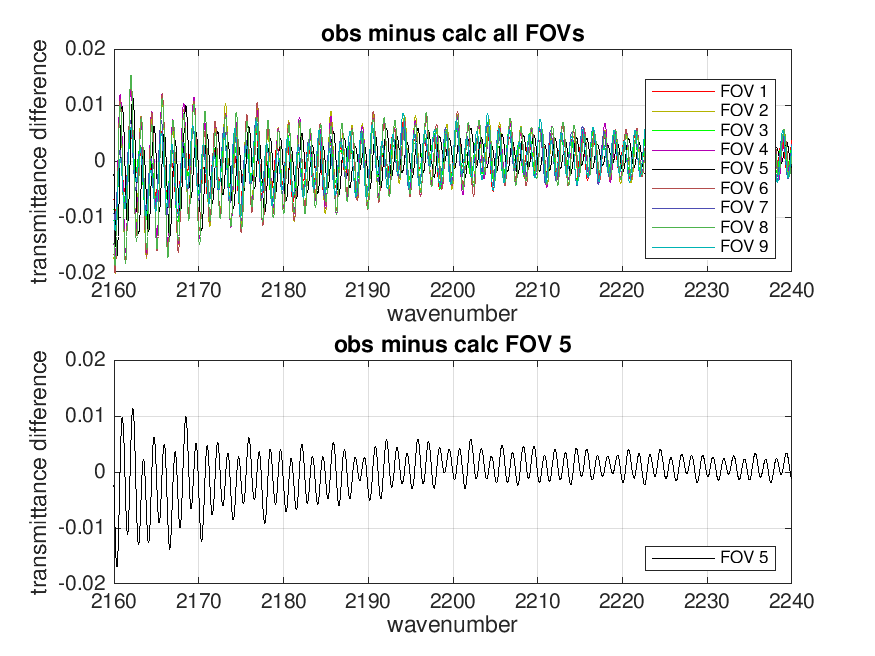
\includegraphics[width=\textwidth]{01-13_pfh_s1_CO/CO_breakout_1.png}
  \end{centering}\vspace{3mm}

Observed minus calculated transmittance for all FOVs and for FOV~5
alone, over the fitting interval.

\end{column}
\begin{column}{0.5\textwidth}  
  \begin{centering}
  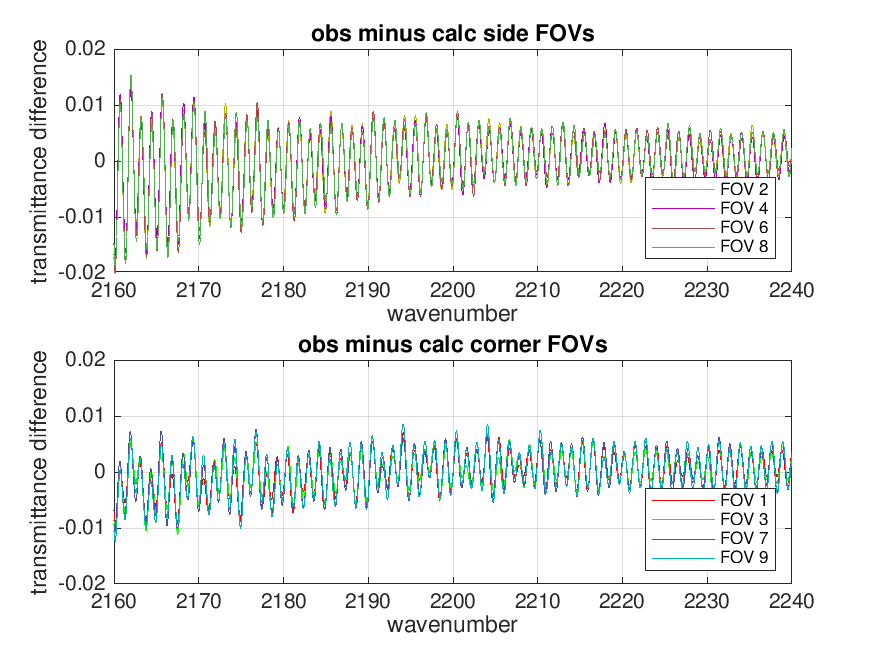
\includegraphics[width=\textwidth]{01-13_pfh_s1_CO/CO_breakout_2.png}
  \end{centering}\vspace{3mm}

Observed minus calculated transmittance for side and corner FOVs,
over the fitting interval.

\end{column}
\end{columns}
\end{frame}
%----------- slide --------------------------------------------------%
\begin{frame}[fragile]
\frametitle{CO side 1 tabulated residuals}

  metrology laser absolute residuals, ppm
\begin{semiverbatim}\scriptsize
      3.62     8.14    14.85         7   4   1
      1.68     5.81    12.01         8   5   2
      3.49     7.23    12.66         9   6   3
\end{semiverbatim}

  metrology laser relative residuals, ppm
\begin{semiverbatim}\scriptsize
     -2.20     2.32     9.04         7   4   1
     -4.13     0.00     6.20         8   5   2
     -2.32     1.42     6.85         9   6   3
\end{semiverbatim}

     regression fitting weights and residuals
\begin{semiverbatim}\scriptsize
 FOV   "a"       "b"     dmin     wmin      wfov
  1   0.989    0.0143   0.0028    14.85   774.2360 
  2   0.990    0.0105   0.0056    12.01   774.2338 
  3   0.984    0.0136   0.0029    12.66   774.2343 
  4   0.992    0.0109   0.0055     8.14   774.2308 
  5   0.991    0.0120   0.0040     5.81   774.2290 
  6   0.993    0.0069   0.0057     7.23   774.2301 
  7   0.994    0.0077   0.0031     3.62   774.2273 
  8   0.998    0.0038   0.0057     1.68   774.2258 
  9   0.990    0.0104   0.0033     3.49   774.2272 
\end{semiverbatim}

\end{frame}
%----------- slide --------------------------------------------------%
\begin{frame}
\frametitle{Conclusions}
\begin{itemize}

  \item We have done a preliminary analysis of the PFH Plateau 21
    CH$_4$, CO$_2$, and CO gas cell tests, and compared these with
    calculated reference truth.  Overall, the results look quite
    good.

  \item The HTBB drift seen in many of the test legs is significant
    but managable with our approach to regression fitting.   The effect
    of the drifts could be reduced with more careful subsetting, if
    needed.

  \item Metrology laser relative residuals are in reasonable
    agreement, and can be reduced further with focal plane
    adjustments.  Metrology laser absolute residuals could be
    reduced with a more judicious choice of neon wavelengh, or 
    possibly by simply using the eng neon value.

\end{itemize}
\end{frame}
%----------- slide --------------------------------------------------%

\end{document}

